%Create a LaTeX template for writing my notes on Parallel Computing with table of contents and proper margin and title
\documentclass[12pt]{article}
\usepackage{amsmath}
\usepackage{amssymb}
\usepackage{graphicx}
\usepackage{float}
\usepackage{hyperref}
\usepackage{listings}
\usepackage{color}
\usepackage{geometry}
\usepackage{fancyhdr}
\usepackage{lastpage}
\usepackage{enumitem}
\usepackage{tikz}
\usepackage{pgfplots}
\usepackage{subcaption}
\usepackage{multicol}
\usepackage{lipsum}

% Insert links to websites for references
\newcommand{\weblink}[2]{\href{#1}{\textcolor{blue}{#2}}}



%Make the code formatting look professional and proper
%Show the with some colored background
% Enhanced code formatting for C++
\definecolor{codegreen}{rgb}{0,0.6,0}
\definecolor{codegray}{rgb}{0.5,0.5,0.5}
\definecolor{codepurple}{rgb}{0.58,0,0.82}
\definecolor{backcolour}{rgb}{0.95,0.95,0.92}

\lstdefinestyle{mystyle}{
    backgroundcolor=\color{backcolour},   
    commentstyle=\color{codegreen},
    keywordstyle=\color{magenta},
    numberstyle=\tiny\color{codegray},
    stringstyle=\color{codepurple},
    basicstyle=\footnotesize\ttfamily, % Using monospaced font for code
    breakatwhitespace=false,         
    breaklines=true,                 
    captionpos=b,                    
    keepspaces=true,                 
    numbers=left,                    
    numbersep=5pt,                  
    showspaces=false,                
    showstringspaces=false,
    showtabs=false,                  
    tabsize=2,
    language=C++, % Specifying the language as C++
    morekeywords={constexpr, nullptr, noexcept} % Adding C++ specific keywords
}

\lstset{style=mystyle}
%Make a command to write note
\newenvironment{note}
{
    \begin{center}
    \begin{tikzpicture}
    \node[rectangle, draw=black!50, top color=black!10, bottom color=black!10, rounded corners=0.5cm, inner xsep=0.5cm, inner ysep=0.5cm] 
    \bgroup
    \begin{minipage}{0.9\textwidth}
}
{
    \end{minipage}
    \egroup;
    \end{tikzpicture}
    \end{center}
}
\setlength{\headheight}{14.49998pt}

\pagestyle{fancy}
\fancyhf{}
\rhead{Page \thepage \hspace{1pt} of \pageref{LastPage}}
\lhead{Parallel Computing}
\renewcommand{\headrulewidth}{1pt}
\renewcommand{\footrulewidth}{1pt}

\pgfplotsset{compat=1.18}
\begin{document}
\title{Notes on Parallel Computing}
\author{Nihar Shah}
\maketitle
\newpage
\tableofcontents
\newpage
\begin{note}
    Here it has been assumed that as a prerequisite, the reader has a basic understanding of C programming language 
    and familiarity with Basics of Computer Architecture.
\end{note}

\section{Introduction}
Moore's Law states
\begin{equation}
    \text{The number of transistors in a dense integrated circuit doubles approximately every two years.}
\end{equation}
This law has been true for the past 50 years. This has led to the increase in the number of cores in a processor.
\begin{figure}[H]
    \centering
    \includegraphics[width=0.8\textwidth]{images/moore.png}
    \caption{Moore's Law Graph}
\end{figure} 
But computing power is saturating. The power consumption is increasing and the heat dissipation is becoming a problem.
Moore's Law is not sustainable. The solution to this problem is parallel computing. 
Parallel Computing is the use of multiple processors to perform a computation. It is a form of computation in which many calculations are carried out simultaneously, operating on the principle that large problems can often be divided into smaller ones, which are then solved concurrently.
It leads to Faster execution times from days or months to hours or seconds. Example: Climate Modelling,
Bioinformatics, Computational Fluid Dynamics, etc.
The large amount of data can be processed in parallel. Example: Google, Facebook, process billions of requests per day.
Parallelism cannot be achieved in all problems. It is not always possible to divide the problem into smaller problems. But it is
more natural for certain kinds of problems. Example: Climate Modelling.

Because of the Computer Architecture trends the CPU Speeds have saturated and thus slow memory bandwidth is the bottleneck.
Parallelism helps in data transfer Overlap.

\section{Classification of Architectures - Flynn's Taxonomy}
Flynn's Taxonomy is a classification of computer architectures based on the number of instruction streams and data streams.
\begin{itemize}
    \item SISD - Single Instruction, Single Data (Serial Computers)
    \item SIMD - Single Instruction, Multiple Data
    \item MISD - Multiple Instruction, Single Data
    \item MIMD - Multiple Instruction, Multiple Data
\end{itemize}
\subsection{SIMD - Single Instruction Multiple Data}
It uses vector processors and processor array. In this, a single instruction is executed on multiple data elements simultaneously. 
\begin{itemize}
    \item Vector Processors - They are capable of executing a single instruction on multiple data elements simultaneously.
    \item Processor Array - It is a collection of processors that work in parallel on different data elements.
\end{itemize}
For example, CM-2, Cray-90, Intel Xeon Phi, Intel -vector instructions (1028 bytes), etc.
\begin{figure}[H]
    \centering
    \includegraphics[width=0.8\textwidth]{images/simd.png}
    \caption{SIMD Architecture}
    \label{fig:simd}
\end{figure}
\href{http://www.llnl.gov/computing/tutorials/parallel_comp/}{Link to Parallel Computing Tutorial}
This link provided by LLNL provides a good tutorial on parallel computing for more information. 
Consider the figure \ref{fig:simd}. Say two vectors A and B are given of size n (i.e. n elements). The operation is to perform 
a element-wise multiplication between the two given vectors. We are given n processors (from P1,...,Pn) Then, in case of SIMD architecture we will pass 
say ith element of the vector to the ith processor i.e. the first processor will get the first element of the vector,
the second processor will get the second element of the vector and so on. Then the processor will simultaneously with time
start executing the same instruction on the data element that it has been given. So as shown in the figure \ref{fig:simd}, 
all the processors will simultaneously load the data element i.e. ith processor will load the ith element of the vector A.
P1 will load A(1), P2 will load A(2) and so on Pn will load A(n). Then they will simultaneously execute the next instruction to load the data element of the vector B. 
Thus, the ith processor will load the ith element of the vector B i.e. P1 will load B(1), P2 will load B(2) and so on Pn will load B(n). 
Then, once the data has been loaded, the processors will simultaneously execute the next instruction to multiply the data elements that they have loaded.
Thus, P1 will multiply A(1) and B(1), P2 will multiply A(2) and B(2) and so on Pn will multiply A(n) and B(n). 
Then, the processors will simultaneously execute the next instruction to store the element in the result vector C. The ith processor will store the result in the ith element of the vector C.
Thus, P1 will store the result in C(1), P2 will store the result in C(2) and so on Pn will store the result in C(n).
Thus, the SIMD architecture is used to perform the element-wise multiplication of two vectors in parallel. This is how the SIMD Architecture works.
\subsection{MISD - Multiple Instruction Single Data}
This is not very common. It is used in fault-tolerant systems. In this, multiple instructions are executed on the same data.
Some of the examples are:
\begin{itemize}
    \item Fault-tolerant systems
    \item Redundant systems
    \item N-modular redundancy
    \item Cryptography - Multiple algorithms to crack same data
\end{itemize}
\subsection{MIMD - Mutliple Instruction Multiple Data}
In this, multiple instructions are executed on multiple data elements. It is the most common architecture.
Some of the examples are IBM SP, most supercomputers, cluster, Computational grids, etc..
At a given time step different processors can execute different instructions on different data elements.
\begin{figure}[H]
    \centering
    \includegraphics[width=0.8\textwidth]{images/mimd.png}
    \caption{MIMD Architecture}
    \label{fig:mimd}
\end{figure}
As shown in figure \ref{fig:mimd}, each of the processor P1, P2, ..., Pn can execute different instructions on different data elements simultaneously in time.
P1 is doing element wise multiplication, P2 is running a completely different instruction simultaneously on completely different data elements and so on.
Thus, MIMD architecture is used to perform different instructions on different data elements in parallel. This is how the MIMD Architecture works.

\section{Classification based on Memory}
\begin{itemize}
    \item Shared Memory
    \item Distributed Memory
\end{itemize}
\subsection{Shared Memory}
In this, all the processors share the same memory. It requires special computer architecture for memory management (explained later). 
It is easier to program.
\begin{figure}[H]
    \centering
    \includegraphics[width=0.8\textwidth]{images/shared_memory.png}
    \caption{Shared Memory Architecture}
    \label{fig:shared_memory}
\end{figure}
As shown in figure \ref{fig:shared_memory}, in this the n processors share the same physical address space i.e.
say the address is 0x7FFF5FBFFD98 then, whenever a processor accesses the address 0x7FFF5FBFFD98 then it refers to the same physical address location in the memory 
for all the processors P1, P2, ..., Pn i.e. thus address 0x7FFF5FBFFD98 is at the same physical location for
all the processors. Thus, any of the processor can access the address 0x7FFF5FBFFD98 or the address 0x7FFF5FBFFD98 refers to the 
same physical location for all the processors. This is called sharing the same physical address space.
It will be cleared further when you will see Distributed Memory Architecture.
It will be explained in detail later how the shared memory is managed in the computer architecture and thus will clear the doubts about how the shared memory is managed. 
This leads to certain problems in Read and Write and Maintaining Cache Coherence (explained later)
Thus, any communication between the processors can be done thorough this shared memory. 
There are two types of shared memory:
\begin{itemize}
    \item Uniform Memory Access (UMA) - All processors have equal access time to all memory locations.
    \item Non-Uniform Memory Access (NUMA) - Access time depends on the location of the memory.
\end{itemize}
In general, the time taken by the processor to access a memory location depends on the 
distance between the processor and the memory location.
\subsubsection{Uniform Memory Access (UMA)}
In this, all the processors have equal access time to all memory locations. It is easier to program.
\begin{figure}[H]
    \centering
    \includegraphics[width=0.5\textwidth]{images/uma.png}
    \caption{Uniform Memory Access Architecture}
    \label{fig:uma}
\end{figure}
As shown in figure \ref{fig:uma}, all the processors have equal access time to all the memory locations i.e.
the time taken by the processor to access a memory location is same for all the processors. All can be thought of as being at 
the same distance from the memory location. Thus, all the processors have equal access time to all the memory locations.
\subsubsection{Non-Uniform Memory Access (NUMA)}
In this, the access time depends on the location of the memory. It is difficult to program.
\begin{figure}[H]
    \centering
    \includegraphics[width=0.5\textwidth]{images/numa.png}
    \caption{Non-Uniform Memory Access Architecture}
    \label{fig:numa}
\end{figure}
As shown in figure \ref{fig:numa}, each processor might have some portion of shared physical address space that is physically close to it and
therefore accessible to it in less time. Thus, the time taken by the processor to access a memory location depends on the location of the memory.

\subsection{Distributed Memory Architecture}
\begin{figure}[H]
    \centering
    \includegraphics[width=0.5\textwidth]{images/distributed_memory.png}
    \caption{Distributed Memory Architecture}
    \label{fig:distributed_memory}
\end{figure}
As shown in figure \ref{fig:distributed_memory},
If two processors access the same memory address say 0x7FFF5FBFFD98 then they will get different data since 
the physical address space is not shared. Thus, the address 0x7FFF5FBFFD98 refers to different physical locations for different processors.
The only way to access data between processor is by sending and recieving data i.e. message passing.
This is generally preferred when we wish to use very large number of cores.
It is difficult to program.

\subsection{Shared Memory Architectures: Cache Coherence}
Now consider the figure \ref{fig:shared_memory}. As shown in the figure the processors are
connected to the Main Memory via Interconnect. Note that even in case of shared memory architecture individual processors have their own caches.
Now suppose there is a variable X in the Main Memory and the value of X is 5. Now suppose
the processor P1 tries to access the variable X, it will be a Cache miss and hence the value of X will be loaded into the cache of the processor P1.
Now suppose the processor P2 tries to access the variable X, it will be a Cache miss and hence the value of X will be loaded into the cache of the processor P2.
Now suppose the processor P1 changes the value of X to 10, it will be a Cache hit and hence the value of X will be updated in the cache of the processor P1.
Now suppose the processor P2 tries to access the variable X, it will be a Cache hit and hence the value of X used will be the stale value 5.
This is called Cache Coherence Problem. The value of X is not consistent across the caches of the processors.
There are two ways to solve this problem:
\begin{itemize}
    \item Write Update Protocol - Propagate Cache lines to other processors on every write to a processor as well as Global memory.
    Write operation in write update takes longer time because it has to send the data to all the processors.
    In Read operation, write update is better as the update data is there in local caches of the processor, hence its a faster read.
    \item Write Invalidate Protocol - Whenever one of the Processor updates the data it sends a signal to other processor to invalidate the data in the cache. Thus, next time
        if the processor requires that data it will be a cache miss and the data loads from the main memory. Each processor gets the latest data from the main memory.
        In update protocol, the write updates are faster as it is required to send only an invalidate signal to the processors. In write invalidate protocol,
        read operation will be a cache miss: thus requires fetching data from memory.
\end{itemize}
\begin{note}
    In write update protocol, if the data is present in another processor it will get updated regardless of whether that data is going to be used on not 
    by that processor. This does not happen in write invalidate protocol. Thus, more traffic in write update protocol. 
    This is why most of the systems use write invalidate protocol. NOTE: The specific steps of protocols vary from implementation to implementation.
\end{note}

\subsubsection{State Transition Diagram}
\begin{figure}[H]
    \centering
    \includegraphics[width=0.8\textwidth]{images/state_dia.png}
    \caption{State Transition Diagram for invalidate protocol}
    \label{fig:state_transition}
\end{figure}
A cache line can be in either of the three states -Shared (S) - a variable shared by 2 caches,
Invalid (I) - another Processor has updated the data, Dirty (D) - the data has been updated by the processor.
In the figure shown in \ref{fig:state_transition}, the state transition diagram for the invalidate protocol is shown.
The solid lines indicate the Primary action and the dashed lines indicate the Cache coherence protocol action.

Now consider the figure \ref{fig:state_transition}. Suppose the cache line is in the shared state S i.e. the data is shared by at least two caches (i.e. in different processors).
Then if it is read by either of the processors, it will remain in the shared state S indicated by the solid black line. \\
If it is written by one of the the processor, it will go to the dirty state D from shared 
state S for the processor that writes the data as shown by the solid red line from S to D, and because of the cache coherence protocol action, it will go to the invalid state I for the other processor as shown by dashed the red line in the
figure \ref{fig:state_transition} from S to I. \\
If the cache line is in the dirty state D i.e. the data has been updated by the processor, then if it is read/write by the processor, it will remain in the dirty state D as shown by solid black line in the figure \ref{fig:state_transition} from D to D.\\
If the cache line is in the invalid state I i.e. the data has been updated by another processor, then, if it is read by the processor, it will 
be a cache miss and hence the data will be loaded from the main memory and the cache line will go to the shared state S as shown by the solid blue line in the figure \ref{fig:state_transition} going from I to S.
Because of this read, the cache coherence protocol action will be to go from the Dirty state D to the shared state S for the other processor as shown by the dashed blue line in the figure \ref{fig:state_transition} from D to S.\\
If the cache line is in the invalid state I i.e. the data has been updated by another processor, then, if it is written by the processor, it will go to the dirty state D as shown by the solid yellow line in the figure \ref{fig:state_transition} from I to D.
Thus, as a result the processor will send an invalidate signal to all the processors as part of the cache coherence protocol, the cache line which was in Dirty state D for the other processor
will thus become invalid. Thus, the dirty state D will go to Invalid state I for the other processor as shown in figure \ref{fig:state_transition} by a dashed yellow line from D to I. \\
\subsection{Implementation of Cache Coherence Protocols}
\subsubsection{Snooping Protocol}
It is generally used for Bus based architectures. Only one operation 
can be done at a time. All the memory operations are propagated over the bus and snooped.
The idea is that each processor has a specialised cache controller which always snoops onto the bus.
Thus, any write operation in any of the cache is publicly broadcasted onto the bus and thus is known by all the other cache controllers 
of the processors hearing on the bus. Thus, any information related to the cache line present in their cache is invalidated.
But this has a problem that only one operation can be done at a time thus, it is slow and not scalable. It requires specialised cache 
controllers for each processor which increases the cost of architecture. All the data write/read are costly because all the processors are 
continuously writing on bus and other processors are snooping on the bus.
To overcome this problem, the directory based protocol is used.

\subsubsection{Directory Based Protocol}
It is generally used for Network based architectures. It is scalable and faster. It is used in large scale systems.
In the snooping protocol all the other processors even which do not have that data are also snooping on the bus and are listening even though they are not concerned with data.
Hence, a mechanism is required where the invalidate signals are sent only to certain processors. This is done by maintaining a directory for each cache line 
which contains the information about which processors have the data. Thus, the invalidate signals are sent only to the processors which have the data.
Thus, instead of broadcasting memory operations to all the processors, cache coherence operations are propagated only to the relevant processors. 
A centralised directory maintains states of all the cache lines and the processors which have the data.
Consider it has M cache lines and P processors, thus a matrix of $M \times P$ is maintained where each row represents a cache line and each column represents a processor.
The data about which processor contains that cache line is maintained by presence bits (1 and 0s) in the matrix. wherever the presence bit is 1,
it means that the processor has the data and wherever the presence bit is 0, it means that the processor does not have the data.
Thus, any invalidate signal will be sent only to the processor with presence bit as 1. The directory also maintains 
who is the current owner of the cache line. 
Note that this is called a \textit{Full Bit Vector Scheme} where the number of presence bits is of the $\mathcal{O}(M \times P)$.
Huge number of cache lines/processors requires huge amount of memory for storing directory and less memory for storing the actual data. Thus, requires
lots of swaps to memory thus, losing the advantage of parallelism. Ideally, at all times only some of the cache lines will be of interest to only some of the processors. 
Thus, the matrix $M \times P$ is sparse. Thus, a \textit{Sparse Bit Vector Scheme} is used where the number of presence bits is of the $\mathcal{O}(M + P)$.
Here the number of cache lines (m) is much lesser than the total number of cache lines(M) $(M<<m)$ and the number of processors (p) is much less than the
total number of Processors (P). $(p<<P)$. Thus, a limited number of cache lines and processors are of interest at any given time.

\subsection{False Sharing}
A cache is made up of multiple cache lines. All the cache coherence protocols, such as write invalidate, write update deal with the granularity of cache lines and not at the scale of individual variables.
Thus, if a variable is in one of the cache lines of caches of two processors and if one of the processors updates some other variable belonging to the same cache line, then even though 
the variable in the other processor was not updated, since the entire cache line is invalidated, the variable in the other processor will be invalidated. This is called False Sharing.

Let us understand this with an example, Consider modern day caches, a modern day cache lines are of 64 bytes in size. 
Now consider the data to be stored be of double type which takes 16 bytes. Thus, we can store 4 double type variables in a cache line.
Now consider two processors P1 and P2. Suppose a cache line is shared by the processors P1 and P2. 
Now, say P1 updates the first variable out of the four variables stored in that cache line. Now consider a situation 
where P2 does not ever required to read or write the first variable but it requires to read or write the second variable.
But, since P1 updates the first variable of the cache line and as the cache coherence protocols deal with granularity of cache lines and not
of the individual variables, this will lead to the entire cache line being invalidated for the processor P2. Thus, even though the processor P1 deals only with the first variable and P2 deals with only the second variable,
the entire cache line will be invalidated for P2. This is called False Sharing. This leads to unnecessary cache misses and thus, the performance of the system is degraded. Thus, even though these two processors are accessing different variables of the same cache line
i.e. it is not true sharing, since processor P1 deals only with the first variable and processor P2 deals with only the second variable, but still any updating to either of the variable will lead to invalidating the entire cache line for the other processor. 
Thus, it is called False sharing. It unnecessarily introduces cache coherence protocols even though the processors are not sharing the same variable or the same element.

\newpage

\section{Interconnection networks for a Parallel Computer}
Interconnection networks for a parallel computer provide mechanisms for data transfer between processing nodes or between
processor and memory modules. A black-box view of interconnection network consists of n inputs and m outputs. Interconnections networks are build using links and switches.\textbf{Links} are set of wires 
or fibres for carrying information. They limit the speed of propagation because of capacitive coupling, attenuation of signal strength 
which are a function of length of link. \textbf{Switch: }A switch maps input ports to output ports. Degree of a switch is the total number of ports on a switch.
It supports internal buffering when output ports are busy and allows Routing (to alleviate congestion on Network) and 
multicast (same output on multiple ports). There are two type of networks:
\begin{itemize}
    \item Static/Direct Networks - It is point to point communication links among the processing nodes Example: Hypercube, Mesh, Torus, etc.
    \item Dynamic/Indirect Networks - They are connected by switches linking processing nodes and memory banks. Example: Crossbar, Omega, etc.
\end{itemize}
The classification is as shown in figure \ref{fig:class_network}. The diagram on the left shows a Static Network and the diagram on the right shows Indirect Network.
\begin{figure}[H]
    \centering
    \includegraphics[width=0.8\textwidth]{images/class_network.png}
    \caption{Classification of Interconnection Network}
    \label{fig:class_network}
\end{figure}

\subsection{Network Topology}
Network topology is evaluated broadly in terms of cost and scalability with performance.
\subsubsection{Bus-based networks}
It is a shared medium that is common to all node. They are scalable in cost but unscalable in terms of performance.
The cost of the network is thus proportional to the number of nodes p, thus scales as $\mathcal{O}(p)$. The distance between any two nodes in the network is constant $\mathcal{O}(1)$.
Since they broadcast information among nodes, there is a little overhead associated with broadcast compared to point to point message transfer.
The bounded bandwidth places limitation on the overall performance of the network. Example: Intel Pentium and Sun Enterprise servers. The demands for bandwidth can be reduced by cache for
each node i.e. Private data, thus, only remote data is to be accessed through the bus.
This is as shown in figure \ref{fig:bus}.
\begin{figure}[H]
    \centering
    \includegraphics[width=0.8\textwidth]{images/bus.png}
    \caption{Bus-based Network}
    \label{fig:bus}
\end{figure}
The figure at the top shows a bus-based interconnects with no local caches.
The figure at the bottom shows a bus-based interconnects with local memory/caches.

\subsubsection{Cross-bar Networks}
Consider the figure \ref{fig:crossbar}. It connects p processors to b memory banks.
It is a non-blocking network i.e. the connection of a processing node to a memory bank does not block the connection
of any other processing nodes to other memory banks. 
\begin{figure}[H]
    \centering
    \includegraphics[width=0.8\textwidth]{images/crossbar.png}
    \caption{Cross-bar Network}
    \label{fig:crossbar}
\end{figure}
The total number of switching nodes is $\Theta(pb)$. Generally, $b>p$ so that 
all the processors can access some memory bank. Thus as p is increased, the complexity of switching network 
grows as $\Omega(p^2)$. Thus, as number of processing nodes becomes large, switch complexity is difficult to realize
at high data rates. Thus, Cross bar networks are not scalable in terms of cost but are scalable in terms of performance.

\subsubsection{Multistage Network}
Consider the figure \ref{fig:multistage}. It lies between crossbar and bus network topology.
It is more scalable than bus in terms of performance and more scalable than cross bar in terms of cost.
\begin{figure}[H]
    \centering
    \includegraphics[width=0.8\textwidth]{images/multistage.png}
    \caption{Multistage Network}
    \label{fig:multistage}
\end{figure}
\textbf{Omega Network} is a type of multistage network with p number of inputs (p processing node), 
p number of outputs (p memory banks) and log(p) number of stages each consisting of p/2 switches. At any consecutive intermediate stage, 
a link exists between input i and output j according to the following interconnection pattern:
%Write a multi line if else equatoin
\begin{equation}
    \text{j} = 
    \begin{cases}
        2i & 0\leq i\leq p/2-1 \\
        2i+1-p & p/2\leq i\leq p-1
    \end{cases}
\end{equation}
This is called a perfect shuffle i.e. left rotation on binary representation of i to obtain j.
In order to understand, consider the example shown in the figure \ref{fig:shuffle}. The figure shows a perfect shuffle interconnection for eight inputs and outputs.
\begin{figure}[H]
    \centering
    \includegraphics[width=0.8\textwidth]{images/shuffle.png}
    \caption{A perfect shuffle interconnection for eight inputs and outputs}
    \label{fig:shuffle}
\end{figure}
Starting from the first input 000. It should be connected to the output obtained on left rotating the input i.e. 000. 
Thus, as can be clearly seen in the figure it is connected to 000. Similarly, the second input 001 should be connected to the output obtained on left rotating the input i.e. 010.
Thus, as can be clearly seen in the figure it is connected to 010. Similarly, the third input 010 should be connected to the output obtained on left rotating the input i.e. 100. 
It can been seen that there is a connection for 010 to 100 and so on for all the inputs till 111 whose left rotation will be 111 and hence a connection between 111 to 111.
Switching nodes can be in either of the two configurations pass thorugh or cross-over as shown in the figure 
\begin{figure}[H]
    \centering
    \includegraphics[width=0.8\textwidth]{images/switching.png}
    \caption{Pass-through and Cross-over configuration of Switching Nodes}
    \label{fig:switching}
\end{figure}
In figure \ref{fig:switching} the figure on the left shows pass-through configuration of a switching node in which the inputs are sent straight to outputs
and the figure on the right shows cross-over configuration of a switching node in which the inputs are crossed over and sent out.

Now, the number of switches required in each stage is p/2 as a switching element takes two inputs and return two outputs. Thus, 
since there are p inputs, p/2 switches are required in each stage. Thus, the total number of switches required is log(p) * p/2 = $\Theta(plog(p))$.
Recall, that the number of switches required in complete cross bar network scaled as $\Theta(p^2)$ and the number of switching nodes in case of a bus-based network
scaled as $\Theta(p)$. Thus, $\Theta(p)<\Theta(p \log p)<\Theta(p^2)$. This, proves that the 
multistage network is more scalable than the cross bar network in terms of cost and more scalable than the bus network in terms of performance. \\
\\
\textbf{Omega Network}\\
Consider the complete omega network as shown in the figure \ref{fig:omega}.
We now understand the routing scheme of the omega network.
\begin{figure}[H]
    \centering
    \includegraphics[width=0.8\textwidth]{images/omega.png}
    \caption{Omega Network}
    \label{fig:omega}
\end{figure}
Let s be the binary representation of processors that need to write some data to bank t.
Now the bits are written in the binary representation. The most significant bit is the left most bit and the least 
significant bit is the right most bit. Now the routing scheme works as follows, at the first switching node, if the most
significant bits of s and t are the same, then the data is routed in pass-through mode. If bits are different than the data is routed through
cross-over mode. At the second switching node, if the second most significant bits of s and t are the same, then the data is routed in pass-through mode.
If bits are different than the data is routed through cross-over mode. This is done for all the bits of s and t, by repeating over 
next switching stage using the next most significant bit. In this way, it uses all log p bits in the binary representation of s and t.

For example, consider a message to be passed from 010 to 111.
As shown in the figure \ref{fig:omega} by dashed lines. As the message reaches the first switching elements because the most significant bits of 010 and 111 are different
the message is routed through cross-over mode. As the message reaches the second switching elements because the second most significant bits of 010 and 111 are the same it 
is routed through pass-through mode. As the message reaches the third switching elements because the third most significant bits of 010 and 111 are different 
the message is routed through cross-over mode. Thus, the message is passed from 010 to 111. \\
Consider another example, consider a message to be passed from 110 to 100. 
As shown in the figure \ref{fig:omega} by solid lines. As the message reaches the first switching elements because the most significant bits of 110 and 100 are the same
the message is routed through pass-through mode. As the message reaches the second switching elements because the second most significant bits of 110 and 100 are different it
is routed through cross-over mode. As the message reaches the third switching elements because the third most significant bits of 110 and 100 are the same
the message is routed through pass-through mode. Thus, the message is passed from 110 to 100.\\
Now consider the case where both of the messages in the above examples were to be passed from 010 to 100 and 110 to 111 simultaneously.
As shown in the figure \ref{fig:omega} by solid and dashed lines. In the case when the processor two and six are communicating simultaneously
then one may disallow access to another memory bank the another processor. This is because they have a common link in the routing scheme shown by AB in the figure \ref{fig:omega}.
This property is called \textbf{blocking networks}.

\subsubsection{Completely Connected Networks}
In this, each node has a direct communication link to every other node in the network. A node can send a message to another node
in a single step, since a communication link exists between them. 
It is a static counter part of crossbar switching networks as the connection between any input/output pair does not block communication between any other pair.
For example, a completely connected network of eight nodes is as shown in the figure \ref{fig:complete}.
\begin{figure}[H]
    \centering
    \includegraphics[width=0.6\textwidth]{images/completelyconnected.png}
    \caption{Completely Connected Network}
    \label{fig:complete}
\end{figure}

\subsubsection{Star Connected Network/Star Topology}
In this, all the nodes are connected to a central node. The central node acts as a switch to connect the nodes.
\begin{figure}[H]
    \centering
    \includegraphics[width=0.4\textwidth]{images/star.png}
    \caption{Star Connected Network}
    \label{fig:star}
\end{figure}
As shown in the figure \ref{fig:star}. Every other processor has a communication link connecting it to this processor. It is thus similar to 
a shared bus. Here, the central processor thus acts as a bottleneck.

\subsubsection{Linear Arrays, Meshes and k-d Meshes}
Linear arrays are as shown in figure \ref{fig:linear}. It is a one-dimensional array of processing nodes. Each node is connected to its immediate neighbours.
\begin{figure}[H]
    \centering
    \includegraphics[width=0.6\textwidth]{images/lineararrays.png}
    \caption{Linear Array}
    \label{fig:linear}
\end{figure}
As shown in the figure \ref{fig:linear} there are two possible cases, the left figure shows a linear array with no wraparound links. It is a 
static network in which each node (except the two nodes at the ends) has two neighbors, one each to its left and right.
The right figure shows a linear array with wraparound links also called a 1D torus. The wraparound links connect the last node to the first node and the first node to the last node.
The ring has a wraparound connection between the extremities of linear array. Each node has two neighbors in this case.\\
\textbf{2D Mesh}\\
It is a linear array extended to 2D as shown in the figure \ref{fig:2dmesh}
\begin{figure}[H]
    \centering
    \includegraphics[width=0.8\textwidth]{images/mesh.png}
    \caption{Mesh}
    \label{fig:2dmesh}
\end{figure}
It has $\sqrt{p}$ nodes in each direction. As shown in the figure there are three possible cases for a 2D mesh.
The leftmost figure shows a 2D mesh with no wraparound links. In this each (i,j) node is connected to (i+1,j),(i,j+1),(i-1,j),(i,j-1).
It can be laird out in 2D space. A variety of regulatory structure computations map naturally to 2D. 2D mesh were often used as interconnects in parallel machines.\\
The middle figure shows a 2D mesh with wraparound links. It is also called a 2D Tori.\\
The rightmost figure is a 3D Cube with no wraparound which is a generalization of 2D mesh to 3D. In this, each node is connected to six other nodes, 
two along each of the three dimensions. 3D simulations can be mapped naturally to 3D.\\
\textbf{General Class of k-d meshes}\\
It is a class of topologies with d dimensions and k nodes along each dimension. Thus, in total kd nodes.
A 1D linear arrays is a special case of a k-d mesh with d=1. A 2D mesh is a special case of a k-d mesh with d=2.
A hypercube has two nodes along each dimensions and has $\log_2 p$ dimensions. It is thus, written as 2-log mesh.
A d-dimensional hypercube is constructed by connection two (d-1) dimensional hypercube as shown in the figure \ref{fig:hypercube}.
\begin{figure}[H]
    \centering
    \includegraphics[width=0.8\textwidth]{images/hypercube.png}
    \caption{Hypercube}
    \label{fig:hypercube}
\end{figure}
The hypercubes follow a numbering scheme which is useful later on for writing many parallel algorithms. 
Number the nodes then place the two d-1 dimensional (p/2 nodes) hypercubes side by side. Prefix one with 0 and the other with 1.
\textbf{Property: The minimum distance between two nodes is given by the number of bits that are different in two labels}. For example,
0110 and 0101 are different in two bits. the third and fourth place bits. Thus, the minimum distance between them is two link apart. This property can 
be used for deriving parallel algorithms for hypercube architecture.
A 4D hypercube with 16nodes is as shown in the figure \ref{fig:4dhypercube}
\begin{figure}[H]
    \centering
    \includegraphics[width=0.8\textwidth]{images/4dhypercube.png}
    \caption{4D Hypercube}
    \label{fig:4dhypercube}
\end{figure}

\subsubsection{Tree Based Networks}
It is a hierarchical network. It is a tree with a root node and each node has a parent and children
as shown in the figure \ref{fig:tree}.
\begin{figure}[H]
    \centering
    \includegraphics[width=0.6\textwidth]{images/tree.png}
    \caption{Tree Based Network}
    \label{fig:tree}
\end{figure}
Note that there is only one path between any pair of nodes.
IN the figure \ref{fig:tree}, the left figure shows a Static Tree Network where each processing element is at 
each node of the tree. The right figure shows a Dynamic Tree Network where the nodes at intermediate level
are switching nodes, and the leaf nodes are processing elements.\\
\textbf{Routing: }Source sends the message up the tree until it reaches the node at the root of the smallest sub tree containing both the 
source and destination nodes. Then the message is routed down the tree towards the destination node.
At higher levels of tree, example, nodes in left sub tree of a node communicate with nodes in right tree, root node must handle all the messages. This leads to
communication bottleneck. It is solved by dynamic tree called Fat Tree as shown in figure \ref{fig:fattree} by increasing the number of connection links and switching nodes close to the root.
\begin{figure}[H]
    \centering
    \includegraphics[width=0.8\textwidth]{images/fattree.png}
    \caption{Fat Tree with 16 Processing Nodes}
    \label{fig:fattree}
\end{figure}
The processors are arranged in leaves and all the other nodes correspond to switches. Note that here the property that 
the number of links from a node to a children is equal to the number of links from the node to its parent. Thus, the edges become fatter as we traverse up.
Now any pair of processors can communicate without contention : non-blocking network. It has a constant bisection bandwidth networks as 
the number of links crossing the bisection is constant. As shown in the example figure \ref{fig:fattree} a two level fat tree has a diameter of four.
\subsection{Evaluating Static Networks}
The performance of a static network is evaluated in terms of cost, performance and scalability.
\subsubsection{Diameter} 
The diameter of a network is the maximum distance between any two processing nodes in the network. The distance between 
any two processing nodes is defined as the shortest path (in terms of number of links) between them. 
For example, the diameter of a completely connected network is 1 and of the star-connected network is two. The diameter of 
a ring network is $\lfloor p/2 \rfloor$. The diameter of a 2D mesh without wraparound connection is $2(\sqrt{p}-1)$.
The diameter of a 2D mesh with wraparound connection is $2\lfloor\sqrt{p}/2\rfloor$.
The diameter of a complete binary tree is $2\log(\frac{p+1}{2})$ because two communicating nodes may be in seperate subtree of the root node and a message might have to travel
all the way to the root and then down the other subtree.

\subsubsection{Connectivity}
The connectivity of a network is a measure of the multiplicity of paths between any two processing nodes. A network with high connectivity is desirable since it lowers latency of communication resources.\\
\textbf{Arc Connectivity of the network: }The minimum no. of arcs that must be removed from the network to break it into two disconnected network. 
For example, Arc connectivity of Linear array, tree star connected networks is 1. 
For rings, 2D meshes without wraparound is 2. It is 4 for 2D meshes with wraparound. It is d for d-dimensional hyper cubes.

\subsubsection{Bisection Width and Bisection Bandwidth}
\textbf{Bisection Width: }The bisection width of a network is defined as the minimum no. of communication links that must be remove to partition into
two equal halves. For example, bisection width of ring=2. Bisection width of 2D p node mesh without wraparound = $\sqrt{p}$. For a 2D mesh with wraparound bisection 
width = $2\sqrt{p}$. Bisection width of a hypercube, but deconstructing the connection we did to get from $2(d-1)$ dimensional hypercube to 1d dimensions hypercube. Hence, 
p/2 nodes to be cut to separate into two subcubes.\\
\textbf{Channel Width: } No. of bits that can be communicated simultaneously over a link connecting two nodes. Channel width = no. of physical wires in each communication link.
\textbf{Channel rate: }The peak rate at which a single physical wire can deliver bits is called the channel rate.\\
\textbf{Channel bandwidth: }Peak rate at which data can be communicated between the ends of a communication link.
Thus, 
\begin{equation}
    \text{Channel bandwidth} = \text{Channel Width} \times \text{Channel rate}
\end{equation}

\textbf{Bisection bandwidth: }The minimum volume of communication allowed between any two halves of the network.
\begin{equation}
    \text{Bisection bandwidth/Cross section bandwidth} = \text{Bisection Width} \times \text{Channel width}
\end{equation}
It is also a measure of cost as it provides a lower bound on areas in 2D packing and volume in 3D.
Say bisection width =w, lower bound on area in 2D packaging gives $\Theta(w^2)$ and for volume in 3D packaging is $\Theta(w^{3/2})$.
According to it, the hypercubes and completely connected networks are more expensive.

\subsubsection{Cost}
Number of communication links or number of wires required by the network.
For example, linear array =p-1 links to connect p nodes. For, d-dimensional wraparound mesh =dp links.
For a hypercube, $\frac{plog}{2}$ links. 

All of this has been summarise in the following table \ref{tab:static_network}. 
\begin{table}[H]
    \centering
    \begin{tabular}{|c|c|c|c|c|}
        \hline
        Network & Diameter & Bisection Width & Arc connectivity & Cost  \\
        \hline
        Completely connected & 1 & $p^2/4$ & p-1 & $\frac{p(p-1)}{2}$ \\
        Star & 2 & 1 & 1 & p-1 \\
        Ring & $\lfloor p/2 \rfloor$ & 2 & 2 & p-1 \\
        Complete Binary Tree & $2\log(\frac{p+1}{2})$ & 1 & 1 & $p-1$ \\
        Linear Array & p-1 & 1 & 1 & p-1 \\
        2D mesh (no wraparound) & $2(\sqrt{p}-1)$ & $\sqrt{p}$ & 2 & $2\sqrt{p}(\sqrt{p}-1)$ \\
        2D mesh (wraparound) & $2\lfloor\sqrt{p}/2\rfloor$ & $2\sqrt{p}$ & 4 & 2p \\
        Hypercube & $\log p$ & $\frac{p}{2}$ & $\log p$ & $\frac{p \log p}{2}$ \\
        Wraprwound k-array d cube & $d \lfloor k/2\rfloor$ & $2k^{d-1}$ & $2d$ & $dp$ \\ 
        \hline
    \end{tabular}
    \caption{Summary of Static Networks}
    \label{tab:static_network}
\end{table}

\newpage

\section{Graphical Processing Units}
A CPU has at max of 32 Cores and 8 threads per core. It is good for serial processing. Thus, they are called Multi-core architectures.
But for parallel processing, we need more cores. Thus, we need to use GPUs. GPUs have 1000s of cores and are good for parallel processing. Thus, are called Many-Core Architectures.
GPUs consist of a large number of light-weight cores which are not as powerful as CPU Cores. In the early, days before 2014 NVIDIA GPUs were used for gaming and video applications for graphical 
displays. Theses can be done in stages with each stage consisting of independent computations like reading pixels, shading, etc. which can be done in highly parallel manner. Reading of one pixel is 
independent of reading of other pixel. Processing/rendering of pixels can happen simultaneously. Higher no. of cores of GPU helps in processing in real time. Thus,
GPU many-core architectures consisting of light-weight cores as they can perform only simple computations and not very heavy computations are used.
Typically GPU and CPU coexists in a heterogeneous setting. GPUs do not exists in standalone setting. 
A program runs on a CPU(coarse-grain parallelism) and CPU offloads some of the computations to the GPU for light-weight computations (fine-grain parallelism).
NVIDIA's GPU architectures consists of CUDA (Compute Unified Device Architecture) which is a parallel computing platform and application programming interface (API) model created by NVIDIA.
CUDA programming model is based on C/C++ and is used to program NVIDIA GPUs. It is used to write parallel programs that run on the GPU.

GPUs were initially used for gaming (possible to divide up monitor pixels to process 
things in parallel). They are also efficient in Matrix calculations.

\subsection{GPU Architecture}
\begin{figure}[H]
    \centering
    \includegraphics[width=0.9\textwidth]{images/gpu.png}
    \caption{GPU Architecture}
    \label{fig:gpu}
\end{figure}
A GPU Architecture is shown in figure \ref{fig:gpu}.
The GPU Architecture consists of five main components:
\begin{itemize}
    \item TPC - Texture Processing Clusters
    \item SMX - Streaming Multiprocessors
    \item SP - Single Precision (GPU Core)
    \item DRAM - Device RAM (GPU RAM)
    \item ROP - Render Output Unit
\end{itemize}
GPU cores are called Streaming Multiprocessors (SMX).
SP cores are called Single Precision (GPU Core).
Coarse level parallelism tasks execute on SMx which gives fine level parallel tasks to execute on SP.
Thus, promotes coarse and fine level parallelism. For example, the latest NVIDIA Architecture 
Kepler consists of 15 SMX with each of 192 SP cores = 2880 SP cores in total.
The speed of each of the processors is 745 MHz which is much less than that of a CPU.
GPus follow SIMT (Single Instruction Multiple Threads) model.
NVIDIA GPU has L2 cache, common memory and individual caches. Each SMX has its own 32 bit registers
for storing the context of GPU threads. 
Consider the figure \ref{fig:smx} of one SMX, 
the GPU has 65536 registers, 192 SP cores - Single Precision Cores for single precision calculations,
64 DP cores - Double Precision Cores for double precision calculations, 32 Special Function Units (SFUs) -
for certain special function, 32 load/store units for loading data from overall GPU memory to shared memory within 
each SMX, 16 Texture filtering units, Shared Memory of size 6 KB. CUDA gives the programmer freedom to use some of it as shared memory
and some of it as L1 cache. Shared memory is controlled by the programmer and L1 cache is taken care by architecture.

Computations are organised as blocks. Blocks are given to SMX. A block consists of many threads and threads are given to SP cores.
\begin{figure}[H]
    \centering
    \includegraphics[width=0.9\textwidth]{images/smx.png}
    \caption{SMX Architecture}
    \label{fig:smx}
\end{figure}

\subsection{CUDA Memory Spaces}
Consider the figure \ref{fig:cuda_memory} of CUDA Memory Spaces. CPU pushes the relevant data to Global memory to be executed on GPU.
It spawns GPU kernels/function which are executed on SMX. Each thread in SMX loads data from global memory/device memory to shared memory.
\begin{figure}[H]
    \centering
    \includegraphics[width=0.9\textwidth]{images/cuda_memory.png}
    \caption{CUDA Memory Spaces}
    \label{fig:cuda_memory}
\end{figure}
The memory spaces in CUDA are:
\begin{itemize}
    \item Global Memory - It is the main memory of the GPU. It is accessible for read/write by all the threads in all the SMXs. 
    It can also be accessed by host - CPU. for Kepler K40 it is around 12 GB. It has a latency of around 200-400 clock cycle (300 ns)
    \item Constant Memory - It is read only memory. It is used to store constants that are used by all the threads in all the blocks.
    \item Texture Memory - It can be accessed by all threads. It is used to store textures, used for texture mapping. It is used to improve performance of reads that exhibit spatial locality among the threads.
    \item Shared Memory - Each SMX has its own individual memory. It is the memory shared by all the threads in a block executing in a SMX. It is faster than global memory. Shared memory has a latency of 20-30 clock cycles (5 ns). The threads can read/write to this memory.
    \item Local Memory - It is the memory local to each thread, used to store temporary variables. Each thread has read/write access to this memory.
    \item Registers - They are present in each SMX. It is the memory local to each thread. It is used to store the context of the thread. Kepler K40 has 64K registers in each SMX.
\end{itemize}
The host can read/write global, constant and texture memory. GPUs prefer to access data from shared memory than device memory because of latency.

\textbf{Difference between CPU and GPU Threads: }There are a few differences between CPU and GPU threads regarding context switching.
Context switching is much faster in GPUs because state of thread (thread block) stored in shared memory and threads stays till execution completion. Unlike in CPUs
where in case of context switch memory related to that thread gets dumped to main memory or disk. Thus, loading the data for the thread next requires loading data from main memory or disk which is 
slow. Thus, context switching is faster in GPUs as there is no need to bring in any data as it already is loaded in the shared memory. Also, in case
of GPUs the cache is explicitly managed by the programmer. The programmer will have to explicitly bring the frequently accessed data from the device to the shared memory. Unlike
in CPUs where the cache is managed by the hardware.

\newpage

\section{Parallelization Principles}
Parallel programs incur overheads which are not present in sequential programs. They are:
\begin{itemize}
    \item Communication Overhead - Time taken to communicate between processors.
    \item Synchronization Overhead - Time taken to synchronize between processors.
    \item Idling Overhead - Time taken by a processor to wait for other processors.
\end{itemize}
A good parallel program tries to minimise these overheads.

\subsection{Evaluation of Parallel Programs}
The performance of a parallel program is evaluated using the following metrics:
\begin{itemize}
    \item Execution Time $(T_p)$ - Time taken by the parallel program to execute.
    \item Speedup (S) - It is the ratio of time taken by the \textit{best} sequential program to the time taken by the parallel program.
    \[ S(p,n)=\dfrac{T(1,n)}{T(p,n)}\]
    where, $T(1,n)$ is the time taken by the best sequential program and $T(p,n)$ is the time taken by the parallel program with p processors.
    Here, n indicates the data size. If we employ p processors we generally expect the speedup of p i.e. the time taken for execution in parallel to be reduced by p times.
    But, usually, $S(p,n)<p$. This is because of the overheads in parallel programs. The overheads are as discussed due to communication, synchronization and idling.
    \begin{note}
        In some cases we may even get $S(p,n)>p$. This is called Super linear Speedup. A large data in sequential program may not fit in cache, thus there will be a 
        lot of cache misses. But in parallel program, the data is distributed among the processors and thus the data fits in the cache and there are less cache misses.
        Thus, decomposing the problem to p processor then each will require a small part of the data and thus the entire data could fit into caches of all the individual processors
        and thus there will be less cache misses and thus the Speedup for that parallel program will be more than p. This is called Super linear Speedup when the speedup is more than p (expected speedup).
    \end{note}
    \item Efficiency - Now generally, we expect the speed up to be of p times. But, speedup alone does not tell the full picture since the same speedup can be achieved by using different number of processors (Say a speedup of 3 can be achieved by using 3 processors or by using 100 processors).
    Thus, we normalize the speedup by the number of processors to get efficiency. Efficiency is the ratio of speedup to the number of processors. It gives the idea of how efficiently our program uses the processors. A low efficiency implies that the overheads are not handled properly and thus are dominating the execution time.
    \[ E(p,n)=\dfrac{S(p,n)}{p}\]
    Generally, Efficiency is less than 1 but sometimes it can be more than 1 because of the super linear speedup.
    \item Scalability - It is the ability of the program to maintain efficiency as the number of processors increases. This is important because we want to be able to use more processors to solve larger problems. If the efficiency decreases as the number of processors increases then the program is not scalable. 
    Thus, the analysis of how the program behaves with increasing the number of processors p or increasing the problem size n is called scalability analysis. Scalability thus tell limitations of the program and how well the program scales in relation to number of processors and problem size.

    Ideally, we would like the Speedup to be linear i.e. Speedup should increase linearly with increase in the number of processors. But, in reality, the speedup is sub-linear.
    Similarly, we would like the efficiency to remain constant with increase in the number of processors but, in practical it decreases with increase in the number of processors.
    This can be explained by Amdahl's Law.

    \textbf{Amdahl's Law: }The performance improvement to be gained from using some faster mode of executing is limited by the faction of the time the faster mode can be used. For the context of parallel programming,
    it states that the speedup of a program is limited by the fraction of the program that cannot be parallelized. Thus, overall speedup is given in terms of fractions of computation time with and without enhancement. Consider a sequential program which takes $t_s$ time, which has $f_s$ part of the program which cannot be parallelized and let 
    $f_p$ be the part of the program that can be parallelized. Thus, in an ideal case the time taken by the parallel program will be addition of $f_st_s$ i.e. time taken by the fraction of the sequential program and $\frac{f_pt_s}{p}$ time taken by the parallelized part of the program. Hence, the total time taken by the parallel program is $f_st_s + \frac{f_pt_s}{p}$.
    Thus, speedup is given by the time taken by the ratio of the time taken by the sequential program to the time taken by parallel program. It is given by:
    \[ S(p)=\dfrac{t_s}{f_st_s+\dfrac{f_pt_s}{p}}=\dfrac{1}{f_s+\dfrac{f_p}{p}}\]
    where, $f_s$ is the fraction of the program that cannot be parallelized i.e. serial and $f_p$ is the fraction of the program that can be parallelized. Thus, the speedup is limited by the fraction of the program that cannot be parallelized.
    This is because not all the operations can be parallelized and some operations are dependent on the previous operations.
    \begin{figure}[H]
        \centering
        \includegraphics[width=0.8\textwidth]{images/amdahl.png}
        \caption{Amdahl's Law}
        \label{fig:amdahl}
    \end{figure}
    It can be seen in the figure \ref{fig:amdahl} that even for highly parallelizable programs ($f_p=0.95$) the speedup curve starts to flatten out as the number of processors increases.
    Thus, it explains that the speedup curves starts flattening out as the number of processors increases. 

    The Amdahl's Law assumes that the problem size is fixed even on increasing the number of processors, thus the fractions $f_s$ and $f_p$ remain constant. 
    But, in reality, the problem size increases with the number of processors. Thus, Gustafson's Law was proposed to address this issue.\\
    \textbf{Gustafson's Law: }Increase the problem size proportionally so as to keep the overall time constant. Here the proportional increase means that the order of computations should increase proportionally to keep the overall time constant
    and not that the the problem size should be increased linearly with the number of processors.\\
    \textbf{Strong Scaling: }The scaling keeping the problem size constant (Amdahl's law) is called strong scaling.\\
    \textbf{Weak Scaling: }The scaling due to increasing the problem size (Gustafson's Law) is called weak scaling.
    \item Isoefficiency - Generally, efficiency decreases with increasing number of processors P and increases with increasing problem size N.
    Isoefficiency is the ability of the program to maintain efficiency as the number of processors increases and the problem size increases. For example, consider the formula for parallel Gaussian elimination in 
    LAPACK package for solving Linear Algebra.
    \[T_{par}(N,P)=\frac{2}{3} \frac{N^3}{P} t_f+ \frac{(3+1/4 \log_2 P)N^2}{\sqrt{P}}t_v+(6+ \log_2 P)Nt_m\]
    \[T_{seq}(N)=\frac{2}{3}N^3t_f\]
    \[E=\frac{T_{seq}(N)}{PT_{par}(N,P)}=(1+\frac{3}{2}\frac{\sqrt{P}(3+1/4\log_2 P)}{N}\frac{t_v}{t_f}+\frac{3}{2}\frac{P(6+\log_2 P)}{N^2}\frac{t_m}{t_f})^{-1}\]
    where, $t_f$ is the time taken for a floating point operation, $t_v$ is the time taken for a vector operation and $t_m$ is the time taken for a memory operation.
    Thus, we can see that from the dominant term in the efficiency equation that as P is increased, N should be increased by $\mathcal{O}(\sqrt{P})$ to keep the efficiency constant.
    Now in Gaussian Elimination function the amount of computations to be carried out is $\mathcal{O}(N^3)$, thus the isoefficiency function is $\mathcal{O}(P\sqrt{P})$. 
    The isoefficiency function is the ability of the program to maintain efficiency as the number of processors increases and the problem size increases. Thus upon increasing the problem size it is
    the number of processors that should be increased to keep the efficiency constant. Thus, the lesser the number of processors to increase with a large increase in the problem size the better the program isoefficiency.
    Thus, the isoefficiency should be as small as possible. Smaller isoefficiency functions imply higher scalability. Consider two parallel programs with isoefficiency functions $W1=\mathcal{O}(P)$ 
    and $W2=\mathcal{O}(\sqrt{P})$. Then the second algorithm is considered to be more scalable since only small amount of processors need to be added. Similarly, an algorithm with an isoefficiency 
    function of $\mathcal{O}(P)$ is highly scalable while an algorithm with quadratic or exponential isoefficiency function is poorly scalable.
\end{itemize}

\newpage

\section{Parallel Programming Classification and Steps}
\subsection{Parallel Program Models}
Classification based on the way the program and Data is written and executed:
\begin{itemize}
    \item Single Program Multiple Data (SPMD): We write a single program and run it on multiple processors. Each processor runs the same program but on different data using processor ids to execute certain parts of data. It is the most common model used in parallel programming.
    \item Mutiple Program Multiple Data (MPMD): Different processors run different programs on different data. It is used in distributed memory systems. For example, used in climate modelling. It is not a very popular model. 
\end{itemize}
\subsection{Programming Paradigms}
Classification based on the way the parallel program uses shared memory model or message passing:
\begin{itemize}
    \item Shared memory Model - If there is a common global memory to access certain data. For example - Threads, OpenMP, CUDA
    \item messaage Passing model - If there is no global memory and the processes explicitly send data whenever required. For example, MPI (Message Passing Interface)
\end{itemize}
\subsection{Parallelizing a Program}
There is no general rule as it all depends on the application. Given a sequential program/algorithm, how to go about producing a parallel version. There are four steps to parallelize a program are:
\begin{itemize}
    \item Decomposition - Identifying parallel tasks with large extent of possible concurrent activity; splitting the problem into tasks that can be executed in parallel.
    \item Assignment - Assign the tasks to the processors and grouping the tasks into processes with best load balancing. i.e. amount of work performed by each of the processes must be equal.
    This is not necessarily done in Decomposition task. It specifies how to group tasks together for a process in order to have balance workload, reduce communication and management cost.
    This is done by structured approaches such as code inspection (parallel loops) or understanding of application. Sometimes the grouping is done statically and sometimes dynamically (i.e. the grouping is done at runtime) based on the load.

    Both decomposition and assignment steps are usually independent of architecture or programming model, but cost and complexity of using primitives may affect decisions.
    \item Orchestration - It is the process of managing the execution of the parallel program. It involves managing the synchronization and communication between the processes. 
    \item Mapping - Mapping the processes to the processors. It is the process of mapping the processes to the processors. It is done in such a way that the processes are mapped to the processors in such a way that the communication overhead is minimized.
\end{itemize}
\subsection{Data Parallelism and Data Decomposition}
\textbf{Data Parallelism: }Given data is divided across the processing entites. \textbf{Owner computes own:} Thus, each process own and computes a portion of the data, it decides which data to communicate between other processes.
This is called owner computes rule. The data is divided into chunks and each chunk is assigned to a process. This is called data parallelism where the data is divided across the processing entities and thus the parallelism is dictated by the data. 

\textbf{Domain Decomposition: }Multi-dimensional domain in simulations divided into subdomains equal to processing entities is called domain decomposition.
The given P processes are arranged in multi-dimensions forming a process grids. Consider the figure \ref{fig:domain}.
\begin{figure}[H]
    \centering
    \includegraphics[width=0.8\textwidth]{images/domain.png}
    \caption{Domain Decomposition}
    \label{fig:domain}
\end{figure}
It shows that if the process grid is arranged as a $1 \times 5$ grid than the 2D domain can be decomposed using the process grid as shown 
and the domain is divided into 5 equal parts. Each process is assigned a part of the domain. The domain decomposition is done in such a way that the communication between the processes is minimized.
Similarly, same concept can be applied for a 3D domain as well as shown in the figure \ref{fig:domain} shows many such ways for decomposing the domain (data) based on different arrangements of process grids.
For a given process gird we decompose the domain so as to map the domain onto process grid such that the communication between the processes is minimized.

\subsection{Data Distributions}
For dividing the data in a dimension using the processes in a dimension, data distribution schemes are followed. 
Common data distributions are:
\begin{itemize}
    \item Block Distribution - The data is divided into blocks and each block is assigned to a process. It is the simplest form of data distribution. It is used when the data is uniformly distributed.
    \item Cyclic Distribution - The data is distributed in a cyclic manner. It is used when the data is not uniformly distributed.
    \item Block-Cyclic Distribution - It is a combination of block and cyclic distribution. It is used when the data is not uniformly distributed.
\end{itemize}
For example, consider the figure \ref{fig:data_distribution}. 
\begin{figure}[H]
    \centering
    \includegraphics[width=0.8\textwidth]{images/data_distribution.png}
    \caption{Data Distribution}
    \label{fig:data_distribution}
\end{figure}
Here, it can be seen that the process grid is arrange as a $2 \times 3$ grid and the blocks of data are distributed in a cyclic manner.

\subsection{Task Parallelism}
We decompose into tasks that can be executed in parallel. It is used when the data is not uniformly distributed.
The independent tasks are identified and mapped to different processors. The tasks are grouped by a process called mapping. 
Here, we are trying to achieve two objectives - balance the groups and minimize inter-group dependencies.
This is represented as a Task graph. For example, consider the task dependency graph shown in figure 
\ref{fig:task_graph}.
\begin{figure}[H]
    \centering
    \includegraphics[width=0.8\textwidth]{images/task_graph.png}
    \caption{Task Dependency Graph}
    \label{fig:task_graph}
\end{figure}
Each node shown represents a task. In general a task can be a statement or a block of statements in a program. 
Suppose, independent tasks follow a tree like parallelism as shown in figure \ref{fig:task_graph}.
The 8 tasks at the bottom are independent and then they are merged to form 4 tasks and then 2 tasks and then 1 task.
Suppose we wish to map this tasks to 8 processors. So, we can map the 8 tasks to 8 processors. Then to merge the tasks we assign it to one of the 
processor as shown in figure \ref{fig:task_graph}, this allows as one of the processor already has the data and the other processor 
can directly access the data from the processor which has the data. Thus, the communication overhead is minimized and similarly for the other tasks.
In general, assigning a task graph to processors is an NP complete problem. Thus, we use heuristics to assign the tasks to the processors.

\subsection{Orchestration}
It is the process of managing the execution of the parallel program. It involves managing the synchronization and communication between the processes.
\subsubsection{Maximizing data locality: }
It is the process of maximizing data locality in a processor and avoid unnecessary communication. Thus, it is about \textbf{minimizing the volume of data exchange}.
(like not communicating intermediate results) or \textbf{Minimizing the frequency of interactions - packing}.
For example, say to compute parallel dot products. Say we have two vectors A and B and we wish to find dot product between two. It requires 
multiplying the corresponding elements of the two vectors and then summing them up. Thus, we can do the multiplication part in parallel across various processes or various threads.
Now the communication part can be done in two ways - either we can communicate the intermediate results to the master processor and then sum them up or we can sum them up in the individual processors and then communicate the final result to the master processor.
The second approach is better as it minimizes the volume of data exchange. Thus, the orchestration is about minimizing the volume of data exchange and \textbf{minimizing the frequency of interactions}. Thus, structuring the communication in such a way that the communication overhead is minimized.
Point to point communication between two processors involves latency and bandwidth. The latency is the time taken to establish the connection between the two processors and the bandwidth (measured in MB/s) is the rate at which the data can be communicated between the two processors. By minimizing the frequecny of interactions we can minimize the overall delay i.e. latency.
For example, consider that a processor is required to send 10 arrays to another processor, then in order to minimize the frequency of interactions 
we can pack all the 10 arrays into one packet and send it to the other processor. In sending 10 arrays together to another processor we require to establish connection only once, thus the delay because of latency
occus only once but in case if we send it as 10 different arrays, we would be required to establish communication between the processors each time which would mean delay due to latency each time. 
Thus, Packing will minimize the frequency of interactions and thus the overall delay. This idea is called 
\textbf{packing}. Note that in this case the volume of data remains the same in both the cases 
but the frequency of interactions is minimized in the second case.

\subsubsection{Minimizing contention and hotspots: }
(Avoiding communication bottlenecks) Do not use the same communication pattern with the other processes in all the processes.
For a given communication pattern, following a certain order will incur a communication bottleneck while following a different order will not incur a communication bottleneck and this can affect the performance.
For example, consider a situation where every process communicates data with every other process.
This is as shown in table \ref{tab:communication}.

\begin{table}[H]
    \centering
    \begin{tabular}{|c|c|c|c|c|c|}
        \hline
        Process & A & B & B & D & E \\
        \hline
        A & - & 2 & 3 & 4 & 5 \\
        B & 1 & - & 3 & 4 & 5 \\
        C & 1 & 2 & - & 4 & 5 \\
        D & 1 & 2 & 3 & - & 5 \\
        E & 1 & 2 & 3 & 4 & - \\
        \hline
    \end{tabular}
    \caption{Communication Pattern}
    \label{tab:communication}
\end{table}

In the table \ref{tab:communication}, 
the communication takes place according to the rule that for each of the processor at time=t, it communicates with t if ($t\neq id$).
Thus, starting from time $t=0$, for Processor A ($id=0$), it won't communicate to anyone else since its $t=id$, for processor B ($id=1$), at time $t=0$
it will communicate (since $t\neq id$) with Processor A.
Similarly for processor C, at time $t=0$, it will communicate (since $t\neq id$) with processor A and so on for Processors D and E, at time $t=0$ they will communicate with Processor A. 
Similarly, at $t=1$, Processor A will communicate with Processor B, for processor B, it will not communicate since ($t =id$), for Processor C it will communicate with Processor B at time $t=1$ and so on for other processors.
This is followed for all the processors at all the time steps.
Now see that at some timestep t all the processors will communicate to processor with $id=t$. This will result in communication bottleneck, although it looks like the processors are communicating in parallel,
but at some timestep t all the processors will communicate to the same processor and thus the communication bottleneck will occur. Even at the hardware level because of the switches and common network links, it can receive only one package at a time.
Now as the number of processes increase say to a 1000, then at some time step t all 999 processes will try and communicate with one of the process at some time step t. Thus leading to communication bottleneck.
The solution is to come up with an algorithm where each process follows a different order in which it communicate with the processes so that at no time step all of them end up communicating with the same processor.
This is called \textbf{minimizing contention and hotspots} which refers to avoiding use of the same communication pattern with the other processes in all the processes.

\subsubsection{Overlapping computations with interactions}
One of the solutions is \textbf{Overlapping computations with interactions}. The idea is to split communication into phases into two parts: one part in which the computations depend 
on  the communicated data (type 1) and second is computations that do not depends on communicated data (type 2). While communicating for type 1 perform computations for type 2.
This can be done especially on the receiver side which do not depend on the communicated data and thus can perform the computation. In other words, the computations are being overlapped with the communications.

\subsubsection{Replicating data or computations }
Balancing the extra computation or storage cost with the gain due to less communication.
For example, consider two processes 0 and 1. 0 computes a matrix A by doing an outer product of two vectors (say a and b) and then distributed this matrix A to process 1.
Then processes computes with their own part of the matrix. 
Instead of his approach, we can replicate the vectors a and b to process 1 and then process 1 can compute the matrix A by itself. This will reduce the communication overhead 
since it will be a lightweight communication compared to sending a part of the Matrix A. But, this will increase the computation overhead since the process 1 will have to compute the matrix A by itself.
Now after both of them compute the matrix A, they can work on their respective parts of the matrix. Depending on the vector sizes instead of computing half of the matrix which could be very huge in size,
we are communicating only the vectors thereby reducing the communications. This is called \textbf{Replicating data or computations} as we are replicating the data and computations to reduce the communication overhead. Here, 
both of the processes end up replicating the data and computations by computing the matrix A to reduce the communication overhead. Ultimately, it all depends on the computation cost and communication cost and the trade-off between them.

\subsection{Mapping}
Mapping the processes to the processors. 
Which process runs on which particular processor.
\begin{itemize}
    \item \textbf{Network topology and communication pattern: }It can depend on network topology and communication pattern of processes. The aspect of mapping the communication pattern to the network topology in an intelligent way plays an important role in the performance of the parallel program.
          For example, consider a 2D mesh network topology. The processes are arranged in a 2D grid and the communication pattern is such that each process communicates with its neighbours. Then we would like to do a natural mapping i.e. map the 
            processes to the processors in such a way that the processes which communicate with each other are mapped to the processors which are close to each other. This will reduce the communication overhead as the communication between the processes will be faster.
          
    \item \textbf{Heterogeneous systems: }On processor speeds in case of heterogeneous systems (different processors have different speeds). In case of homogeneous systems all the processors have same speed and communication cost is same.
          In case of heterogeneous systems the communication cost as well as processor speed is different for different processors and thus the mapping can depend on the communication cost. For example, consider a system with 2 processors A and B. Processor A is faster than processor B.
            Now, if the communication cost between processor A and B is less than the computation cost of processor B then it is better to map the process which communicates with processor B to processor A. This is because the communication cost is less than the computation cost of processor B. Thus, we wish to map the processes 
            to processors in such a way that heavy compute tasks are mapped to faster processors and light compute tasks are mapped to slower processors.
\end{itemize}
All data and task parallel strategies generally follow static mapping i.e. at the beginning of the program the mapping is done and it remains constant throughout the program.
But, in some cases dynamic mapping is done i.e. the mapping is done at runtime. For example, consider a situation where the load on the processors is not uniform and the load on the processors keeps changing. In such cases, dynamic mapping is done where the mapping is done at runtime based on the load on the processors by the master processor.
The idea here is that a process/global memory can hold a set of tasks. The master processors distributed some tasks to all the processes. Once a processor completes its tasks, it asks the coordinator process for more tasks.
This is referred to as self-scheduling or work stealing, where the processes are scheduled dynamically based on the load on the processors. Here we don't fix the tasks onto the processors but let the processes decide dynamically which tasks to take up.
Thus, even in case of heterogeneous processors, the processes working on a high speed processor can finish tasks quickly and will then steal more work from the slower processors. This is called work stealing.


To summarise the various steps they are as shown in the table \ref{tab:summary}
\begin{table}[H]
    \centering
    \begin{tabular}{|c|c|p{0.5\textwidth}|}
        \hline
        \textbf{Step} & Architecture-Dependent? &  \textbf{Description} \\
        \hline
        Decomposition & Mostly no &  Identifying parallel tasks with large extent of possible concurrent activity but not too much \\
        Assignment & Mostly no & Balance workload; reduce communication volume; Assigning the tasks to the processors \\
        Orchestration & Yes & Reduce non inherent communication via data locality; reduce communication and synchronization cost as seen by the processor; reduce serialization at shared resources; schedule tasks to satisfy dependencies early;
        Managing the execution of the parallel program \\
        Mapping & Yes & Put related processes on the same processor if necessary; exploit network topology; Mapping the processes to the processors \\
        \hline
    \end{tabular}
    \caption{Summary of Steps}
    \label{tab:summary}
\end{table}
As shown in the table \ref{tab:summary}, the decomposition and assignment steps try to identify independent tasks and balance the workload. Once these tasks are fixed and the communication patters are fixed,
the orchestration step tries to minimize the communication overhead and the mapping step tries to map the processes to the processors in such a way that the communication overhead is minimized. The Orchestration and Mapping steps are architecture dependent as they depend on the network topology and the communication pattern of the processes.
The first two steps Decomposition and Assignment are mostly independent of the architecture and are done at the programming level.

\subsection{Example}
Given a 2d array of float values, repeatedly average each elements with immediate neighbours until the difference between two
iterations is less than some tolerance value. Consider a 2d domain with some grid points, we start with some initial values at this grid point and we keep updating the values over time.
For example, it could be solving a heat equation where the heat spreads over a plate, thus the grid points represent temperature at different points on the plate and thus averaging the value reduces the temperature at that point.
So we are looking at how the values of these temperatures evolve over time.

%Add code
\begin{lstlisting}[caption={Parallel Program for Averaging},captionpos=b]
do{
    diff=0.0
    for (i=0;i<n;i++)
        for (j=0;j<n;j++){
            temp=A[i][j];
            A[i][j]=average(neighbours);
            diff+=abs(A[i][j]-temp);
        }
}while (diff>tolerance);    
\end{lstlisting}
Consider the figure \ref{fig:grid} which shows the grid points and the neighbours of the grid points.
\begin{figure}[H]
    \centering
    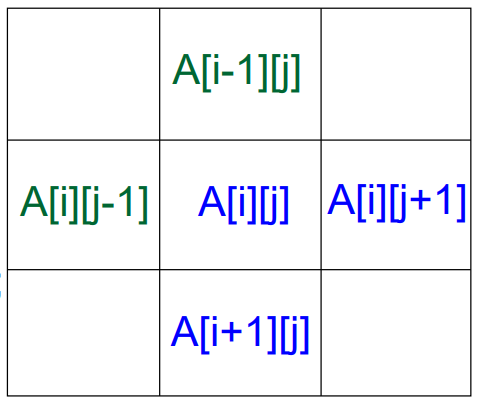
\includegraphics[width=0.6\textwidth]{images/grid.png}
    \caption{Grid Points}
    \label{fig:grid}
\end{figure}
In this we go over all the values of the grid points and update the value of the grid point by averaging the values of the neighbours. We keep doing this until the difference of global variable diff between the two iterations is less than some tolerance value.
There are two methods to solve this problem: one is Jacobi method where we take the values of the neighbour from the previous time step and the other is Gauss-Seidel method where we take the values of the neighbour from the current time step whenever available (for the lower index values we use the latest values and for the higher index values we use the previous values).
Suppose we want to parallelize the program. For the purpose of parallelizing the program we wish to decompose the problem into tasks that can be executed in parallel.
\begin{enumerate}
\item One way is to consider each element in parallel. A parallel process or a parallel thread for each of the element i.e. concurrent task for each element update:
which would require a max concurrency of $n^2$ tasks (for n*n elements in the grid). Practically, this is not feasible as the number of tasks is very large and the overhead of creating and managing the tasks is very high. This many parallel number of threads is not practically possible,
as for larger values of n the number of threads required will be $n^2$, thus many threads would have to be mapped to the same processors and would require a lot of context switching between threads and context switching between the processes which can thus affect the performance.
\item Another way is to consider tasks for elements in anti-diagonal. Note that values in a particular diagonal depends on the values from the previous diagonal but not among the elements in that diagonal.
Now we consider a particular diagonal, for some element in the diagonal for using the Gauss-Siedel method we require the values of the neighbours from the previous diagonal at latest time step and the value from the next diagonal at previous time step. This works out, since we are computing diagonal by diagonal 
starting from the left top corner and moving towards the right bottom corner. Thus, the values of the neighbours are available from the previous diagonal at the latest time step and the next diagonal at the previous time step. Also note that the values of the elements in the diagonal are independent of each other and thus can be computed in parallel.
Thus, we can consider the tasks for the elements in the anti-diagonal and compute the values of the elements in the anti-diagonal in parallel. This way we can reduce the number of tasks to $2n-1$ tasks (for n*n elements in the grid). This is a better approach than the previous approach as the number of tasks is reduced and the tasks are independent of each other and can be computed in parallel.
Note that for the diagonals which are at the ends, will have small number of elements, thus the parallelism will also be very small. This also will have a synchronization const because the processes assigned to a particular diagonal cannot start executing until the earlier diagonals
have finished executing. Thus, the parallelism will be limited by the number of elements in the diagonal and the synchronization cost.
\item What we follow is block distribution of the data. Consider the figure \ref{fig:block} which shows the block distribution of the data.
\begin{figure}[H]
    \centering
    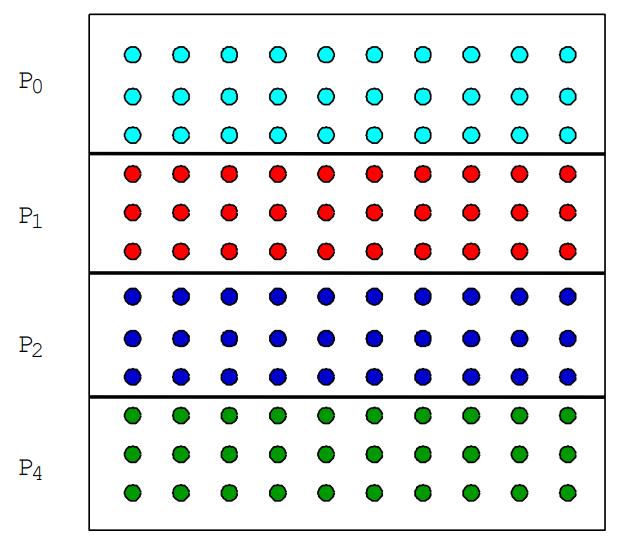
\includegraphics[width=0.6\textwidth]{images/block.png}
    \caption{Block Distribution}
    \label{fig:block}
\end{figure}
In this we have divided the 2d grid across the rows. First set of rows is assigned to P0, the second set of rows assigned to P1 and so on. Each processor will be responsible 
for updating the values of the elements in the rows assigned to it. Now for orchestration step, we try to find out what are the synchronization and communication requirements and we try to ensure correctness and minimize communication and synchronization calls.
It depends on the programming/model architecture - shared memory model/message passing model. 
\end{enumerate}

\textbf{Shared address space/Shared memory model}\\
Now we consider Shared Address space (SAS) version of the above program as shown in lstlisting \ref{lst:shared}.
\begin{lstlisting}[caption={Shared Address Space Version},captionpos=b,label={lst:shared}]
int n, nprocs; /* matri: (n+2 x n+2) elements */
float **A, diff=0;
LockDec(lock_diff);
BarrierDec(barrier1);
main()
begin
    read(n); /*read input parameter: matrix size*/
    Read(nprocs);
    A = malloc(a 2-d array of (n+2) x (n+2) doubles);
    Create(nprocs-1,Solve, A);
    initialize(A); /*initialize the matrix A somehow*/
    Solve(A);
    Wait_for_End (nprocs-1);
end main
\end{lstlisting}
Note that here we are using $n+2$ processors in order to take care of the boundary processors.
Here, the array A will be shared and the main process creates the different processes and then it is solved.
Let us now look at the psuedo code for the Solve function.
\begin{lstlisting}[caption={Solve Function},captionpos=b,label={lst:solve}]
procedure Solve(A) /* solve the equation system*/
    float **A;
begin
    int i, j, pid, done =0;
    float temp;
        mybegin = 1 +(n/nprocs)*pid;
        myend =mybegin+(n/nprocs);
    while(!done) do /* outermost loop over sweeps*/
        diff=0; /*initialize difference to 0*/
            Barriers(barrier1, nprocs);
        for (i=mybeg to myend) do /*sweep for all points of grid*/
            for (j=1 to n) do
                temp=A[i,j]; /*save old value of element*/
                A[i,j]=0.2*(A[i,j]+A[i,j-1]+A[i-1,j]+A[i,j+1]+A[i+1,j]); /* compute average*/
                diff+=abs(A[i,j]-temp);
            end for
        end for
        if(diff/(n*n) < TOL) then done =1;
    end while
end procedure
\end{lstlisting}
Now this particular function is going to be executed by all the processes. But depending on the 
process id different processes will end up processing different parts of the grid. Thus, it uses Single Program Multiple Data Model.
It uses the same single program but executed by different processes on different data.
The $mybegin=1+(n/nprocs)*pid$ and $myend=mybegin+(n/nprocs)$ are the starting and ending points of the grid that the process is responsible for and thus it is calculated based on the process id for each of the processor.
Now all the processes enter the while loop. Here, we have a global variable diff and matrix A which is shared by all the processes.
At the beginning of the loop all the processes synchronize as shown in the code by Barriers.
Each of the processes then execute the statement 11. Although they will be executing the same statement but the beginning and the ending row will differ depending 
on the process id, thus different processes will be executing this code for different sets of rows.
Now, the processes will be updating the values of the elements in the grid and then calculating the difference between the new value and the old value. After taking the average note that they 
update the value of diff, but since diff is a global variable it gets updated by all the processes which is then later on compared with tolerance to determine the end of the loop.
This was just an overview of the program. For understanding the benefits of computing in parallel, we need to understand the importance of parallel statements like barrier.
A barrier is a function call that achieves synchronization calls between the processes. When a particular process calls a barrier, it keeps waiting in the barrier call until all the other processes have reached the barrier call.
Thus, the barrier call ensures that all the processes have reached the barrier call before any of the processes can proceed further. This is important in the above program as we need to ensure that all the processes have completed the computation of the elements in the grid before we can proceed to the next iteration.
This avoids the situation where some of the processes have completed the computation and some of the processes have not completed the computation and thus the processes which have completed the computation will be waiting for the other processes to complete the computation
instead of moving with the computation so as to avoid the use of stale values which are still not updated by the other processors.

\begin{note}
    The matrix A is a global variable and is thus shared by all the processes. But during execution note that the processes are updating
    the values of the elements in the matrix A. Thus, in case when the elements at the boundary of two processors are updated, it may lead to a problem since
    it may happen that the processor may not yet have updated some of the values at the boundary but when the other processor updates the element under its control
    it may use the updated value of the element in some cases and stale value of the element in some cases. Thus, the updates of the elements at the boundary of the processors
    should be done in a synchronized way. This can be achieved in Case of Jacobi method by maintaining a temporary array which is local to each processor, that stores values for the current 
    time step based on the values stored in the global matrix (which contains values at the previous time step). Once all the processes have reached the end of the iteration which can be found using a barrier call.
    Then the temporary matrix will be copied to the global matrix and the next iteration will start. This way the updates of the elements at the boundary of the processors will be synchronized in case of Jacobi method.
    Here, we are ignoring this case for the sake of simplicity and are assuming that this problem is somehow handled internally.
\end{note}

Then we have a waitforend followed by solving matrix A in the code in \ref{lst:shared}.
The waitforend is for the main process waiting for all the processes to finish which can be done by making all the process 
send a synchronization message to the first process which is an All to one communication.
Note that diff variable is a global variable thus is a shared variable which is read and written to by all processes.
Thus, it may result in garbage values since all the processes try to simultaneously read and change a shared variable. This is because of the race conditions
because of context switching at the assembly level language which may result in garbage values.
The solution to this is to use locks. A lock is a mechanism that allows only one process to access the shared variable at a time. Thus, when a process is accessing the shared variable, it locks the shared variable and then
accesses the shared variable and then unlocks the shared variable. This way only one process can access the shared variable at a time.
In computer science, a lock or mutex (from mutual exclusion) is a synchronization primitive. A lock is designed to enforce a mutual exclusion concurrency control policy. This means that only one thread at a time may acquire the lock and all other threads attempting to acquire the lock are blocked until the thread that acquired the lock releases it.
In other words, in order to protect the shared variables by means of this locking mechanisms of mutex locks (mutual exclusion locks) where only that
process which holds the lock will go ahead and execute these statements and it is only when the process releases this lock 
that the other processes can go ahead and execute the statements. This is called mutual exclusion because the processes are mutually
excluding each other and one process gets exclusive access to that part of the code which is called a critical section.
Note that this is also happening with the matrix A which is also a global variable and thus a shared variable. Thus, especially at the boundary values
of the processors, where the values may be updated and read simultaneously, it is important to
use locks to protect those boundary values when you are using shared arrays.

Another way to resolve these is by using temporary matrices which are local to each processor and then copying the values of the temporary matrix to the global matrix after all the processes have completed the computation.
This way the updates of the elements at the boundary of the processors will be synchronized. This is called double buffering.

Note that in the case we are using locking mechanisms, which are very costly and need to be used sparingly,
since each time after the processes updates the value, for updating the value in the diff variable, the processes are waiting for the lock to be released by the other process and then only they can proceed further. 
Note that this happens for each of the grid point updates. 
This can lead to a lot of waiting time and thus the performance of the program can be affected.
So then the question arises, how to reduce the waiting time and the contention for the lock.
Note that diff is needed only for calculating the final global value and to find out whether the convergence condition is achieved or not.
Hence, instead of each process updating this global diff variable on every update of the grid point, we can have a local diff variable for each process which is updated by each process and then at the end of the iteration
the local diff variables of all the processes are added to get the global diff variable. This way the contention for the lock is reduced and the waiting time is reduced since it is only at the time when all the
local variables are added to the global diff variable that the lock is required. This is called reduction operation. Thus, we have reduced the locking overhead from $\mathcal{O}(n^2)$ for each grid point 
update to $\mathcal{O}(p)$ where p is the number of processes. This is a significant improvement in the performance of the program.

Now the updated solve psuedo code is as shown in the listing \ref{lst:solve2}.
\begin{lstlisting}[caption={Updated Solve Function},captionpos=b,label={lst:solve2}]
procedure Solve(A) /* solve the equation system*/
    float **A;
begin
    int i, j, pid, done =0;
    float mydiff, temp;
        mybegin = 1 +(n/nprocs)*pid;
        myend =mybegin+(n/nprocs);
    while(!done) do /* outermost loop over sweeps*/
        mydiff=diff=0; /*initialize difference to 0*/
            Barriers(barrier1, nprocs);
        for (i=mybeg to myend) do /*sweep for all points of grid*/
            for (j=1 to n) do
                temp=A[i,j]; /*save old value of element*/
                A[i,j]=0.2*(A[i,j]+A[i,j-1]+A[i-1,j]+A[i,j+1]+A[i+1,j]); /* compute average*/
                mydiff+=abs(A[i,j]-temp);
            end for
        end for
        lock(diff-lock);
            diff +=mydiff;
        unlock(diff-lock)
        barrier(barrier1,nprocs);
        if(diff/(n*n) < TOL) then done =1; /* checking the terminating condition*/
        Barrier(barrier1,nprocs);
    end while
end procedure
\end{lstlisting}
Note that now in the pseudo code a new local vairable mydiff has been introduced for each of the processes
which is updated by each of the processes and then at the end of the iteration the local mydiff variables of all the processes are added to get the global diff variable
using the locking mechanism as shown in the code \ref{lst:solve2}. See that the statement lock(diff-lock) and unlock(diff-lock) are used to lock and unlock (or releasing the lock) 
the global diff variable respectively
This way the contention for the lock is reduced and the waiting time is reduced since it is only at the time when all the
local variables are added to the global diff variable that the lock is required.
Also note that the barrier call is used to synchronize the processes at the end of the iteration. This is important as we need to ensure that all the processes have completed the computation of the elements in the grid and added 
their value from mydiff is added to global diff before checking the terminating condition in order to proceed to the next iteration.

Now there is another barrier call after we check the terminating condition. This is because in case if the terminating condition is not met then one of the process may 
start executing for the next iteration and see that in the beginning of the iteration set diff=0.
Thus, while the other processes are still checking the terminating condition, 
they may encounter diff=0 in the terminating condition which is wrong. Thus, we add another barrier for letting all the processes
check the terminating condition with the correct diff value and once all the processes are done, then proceed to the next iteration.

Then, the done=1 condition at the convergence point is updated redundantly by all the processes.
Note that the code that does the update is identical to the sequential program.

This is also one of the advantages of a shared memory program over a message passing program.
In a shared memory program, the code that is written is identical to the sequential program and the parallelism is achieved by adding the parallel constructs like locks and barriers.
Thus, the code is easier to write and debug as compared to a message passing program where the code is completely different from the sequential program and the parallelism is achieved by sending messages between the processes.

\textbf{Message Passing Version}\\
Here we cannot assume A to be a global shared array which all the processes can access.
Because there is no concept of shared variable in message passing model. Each process will have to maintain its part of the matrix.
The only way to receive values update by some other processor is by using the explicit message passing between these tow processes.
Thus, we need to send the data to the processes.

We do a domain decomposition to decompose the 2D domain into different processes and each process follows the owner compute rule.
Here we have more communication and on top of that we will be maintaining local data structures because there is no concept of global data structures.
Here, we use something called as ghost rows. This  can be understood as follows. Consider the figure \ref{fig:ghost}.
\begin{figure}[H]
    \centering
    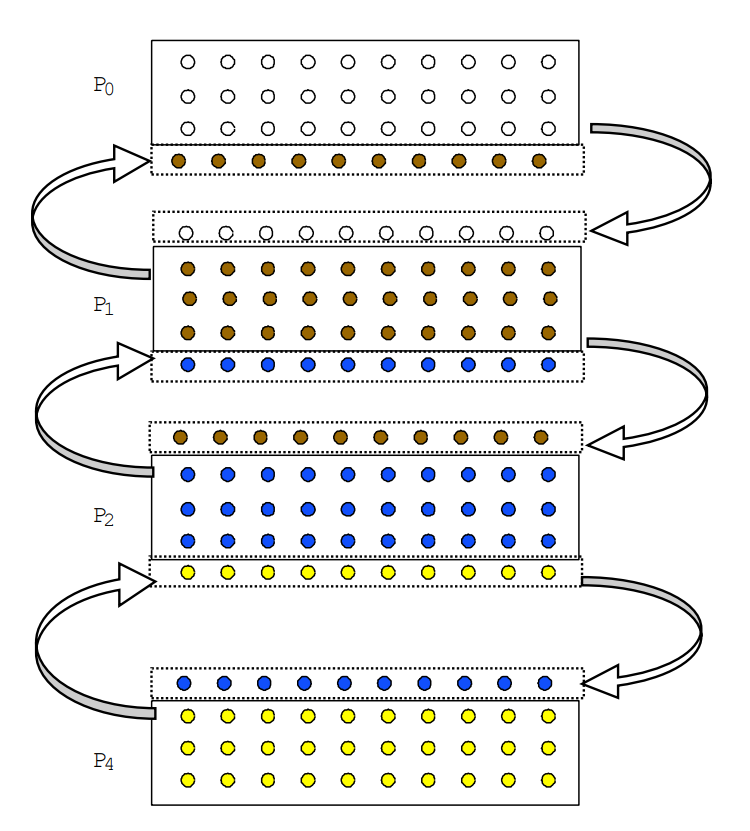
\includegraphics[width=0.6\textwidth]{images/ghost.png}
    \caption{Ghost Rows}
    \label{fig:ghost}
\end{figure}
Here, we have divided the 2D grid into 4 processes as done in the previous case of shared memory model.
Each process is responsible for updating the values of the elements in the rows assigned to it.
Here Each process will have its local array because there is no concept of shared array in orrder to maintain these elements.
In addition each process has an additional ghost row as shown in the figure \ref{fig:ghost}.
These rows are to accommodate the boundary rows coming from other processes. For example, as shown in the figure \ref{fig:ghost},
the process 0 has a ghost row at the bottom which will accommodate the boundary row from process 1. Similarly, the process 1 has a ghost row at the top to accommodate boundary row from process 0
and at the bottom which will accommodate the boundary row from process 2 and so on.
The ghost row values will be used for updating the local values and they will not be updated by the processes themselves.
THe ghost row values will be used just to update the local values of the processes and they will be updated by the processes which own them.
Thus, the name ghost rows. They are also called as halo rows or halo regions or ghost zone regions.
Then each process can imply do sequential computation.

Now consider the following Generating processes code for the message passing version as shown in listing \ref{lst:mpi}.
\begin{lstlisting}[caption={Message Passing Version - Generating Processes},captionpos=b,label={lst:mpi}]
int n, nprocs; /* matrix: (n+2 x n+2) elements */
float **myA;
main()
begin
    read(n); /*read input parameter: matrix size*/
    realead(nprocs);
    A = malloc(a 2-d array of (n+2) x (n+2) doubles);
    Create(nprocs-1,Solve, A);
    initialize(A); /*initialize the matrix A somehow*/
    Solve(A);
    Wait_for_End (nprocs-1);
end main
\end{lstlisting}

Now consider the following Solve function for the message passing version as shown in listing \ref{lst:solve3}
which contains Array allocation and ghost row copying.
\begin{lstlisting}[caption={MPI - Solve Function},captionpos=b,label={lst:solve3}]
procedure Solve(A) /* solve the equation system*/
    float **A;
begin
    int i, j, pid, done =0;
    float mydiff, temp;
    myend=(n/nprocs);
    myA=malloc (array of (n/nprocs) x (n) floats);
    while(!done) do /* outermost loop over sweeps*/
        mydiff=0; /*initialize local difference to 0*/
        if (pid!=0) then
            SEND(&myA[1,0],n*sizeof(float),(pid-1),row);
        if (pid!=nprocs-1) then
            SEND(&myA[myend,0],n*sizeof(float),(pid+1),row);
        if (pid!=0) then
            RECEIVE (&myA[0,0],n*sizeof(float),(pid-1),rpw);
        if(pid!=nprocs-1) then
            RECIEVE(&myA[myend+1,0],n*sizepf(foat),(pid-1),row);
        for (i=1 to myend) do /*sweep for all points of grid*/
            for (j=1 to n) do
                temp=A[i,j]; /*save old value of element*/
                A[i,j]=0.2*(A[i,j]+A[i,j-1]+A[i-1,j]+A[i,j+1]+A[i+1,j]); /* compute average*/
                mydiff+=abs(A[i,j]-temp);
            end for
        end for
        if(pid!=0) then
            SEND(mydiff,sizeof(float),0,DIFF);
            RECIEVE(done,sizeof(int),0,DONE);
        else
            for k=1 to nproces-1 do
                RECEIVE(tempdiff,sizeo(float),k,DIFF);
                mydiff+=tempdiff;
            end for
            if (mydiff/(n*n)<TOL) then done =1;
            for k = 1 to nprocs-1 do
                SEND(done,sizeof(int),k,DONE);
            end for
    end while
end procedure
\end{lstlisting}

In the code \ref{lst:solve3}, the myA is the local array for each of the processes which is used to store the local values of the elements in the grid
for the domain allocated to it (some subset or rows and all columns). These can be done in many ways: one is to make each of the processes read from a file
and the other is to make one of the process can initialize the entire matrix and then distribute it to the various processes.
For the sake of simplicity, let us assume that the processes are somehow able to initialize the matrix.
Inside the while loop, each of the process maintains a local diff value (no concept of shared/global memory since it is a message passing model nothing is shared).
Then, at the beginning of the iteration each processes send their boundary data to the neighbouring processes and the neighbouring processes receive 
this boundary data and store into the ghost rows of their local array. This is done using the SEND and RECEIVE functions as can be seen in the code.
The conditions written here are because the process 0 does not have a process before it and the last process does not have a process after it so 
they do not need to send or receive the boundary data to any processes before and after and need to send and receive data only to the processes that they share a boundary with. 
Here pid is the processid which does from 0 to nprocs-1. Thus, based on the process id the send and recieve blocks will change and 
based on these decisions the processes will change the corresponding send and receive statements. For example from the code we can see that a process with pid not 0 sends 
its top row to a lower rank process and a process with pid not equal to nprocs-1 sends its bottom row to a higher rank process. Then we have the corresponding receive statement for
the same. This way the boundary data is exchanged between the processes and the ghost rows are updated with the boundary data.
Then the processes update the values of the elements in the grid and then calculate the local diff value as done in the sequential code.

This time the diff value is not a global variable but a local variable for each of the processes. 
Then, the processes send their local diff values to the process 0 which is the master process. The process 0 receives the local diff values from all the processes and then adds them to get the global diff value.
Then, the process 0 checks the terminating condition and if the terminating condition is met then it sends the done signal to all the processes and the processes terminate.
This is the message passing version explained in a nutshell using a Psuedocode.

\subsection{Notes on Message Passing Version}
\begin{itemize}
    \item In a shared memory model although there is no explicit communication,
    when a process writes the variable and the other process reads it you can take it as some kind of communication. But the communication 
    is receiving process initiated i.e. when the receiving process receives the data is the communication completed whereas in message passing version
    a process explicitly sends to another process thus it is sender initiated. 
    \item The synchronization in case of Message passing version is implicit. It is not explicitly done using barriers as in the case of Shared memory model
    but the synchronization happens using these communications (denoted by SEND and RECEIVE calls in the program).
    This arises the question whether a deadlock situation can arise due to communications in case for MPI? It may happen in the case when all the processes are waiting for the other process to send something 
    and none of the processes are sending anything. This is called a deadlock situation. Say all the processes execute a RECEIVE statement and until this operation is completed they cannot move on to the next statement to SEND.
    This will lead to a deadlock situation since all the processes are stuck at RECEIVE statement to receive data but none of the processes are sending anything. This can also be though in other way that consider that all the processes execute SEND statement
    and it is such that the processes will move on to the next statement only after it has been received by some other processes. Then in these cases a deadlock situation will happen since all the SEND operations of all the processes will be waiting for each other 
    to execute their RECEIVE statement which will not happen because those processes are also waiting for other processes to consume the message. Thus, all the processes will be at the SEND stage waiting for each other.
    This can be avoided by using non-blocking communication calls. Such a communication is called synchronized communication where we want that a process return from SEND only if the other process begins to receives the message, thus called synchronized communications since the 
    processes are synchronizing. We can try and break the deadlock by one process sending the data and the other process receiving the data.
    \item The communication is done at one in whole rows at the beginning of the iteration, not grid-point by grid-point. Instead of sending rows in each grid point the entire row is sent in one shot.
    \item Note the communication pattern when the mydiff variable is sent from all the processes to the master process and the the master process forms the global value using all this local values. This kind of communication pattern is called All to One communication and is called reduction.
    This is very common operation in parallel programming where all the processes send their local values to the master process and the master process combines all these local values to form the global value. Thus, many parallel programming libraries support automatic functions for reduction.
    Finally, the master process sends the done signal to all the processes which is called One to All communication which is also called a Broadcast operation where one of the process broadcasts a message to all the other processes.
    Thus, we can use the following code by replacing the SEND and RECEIVE operations to broadcast and reduction operations.
    \begin{lstlisting}
    /*communcate local diff values and determine if done, using reduction and broadcast*/
    REDUCE(0,mydiff,sizeof(float),ADD);
    if(pid==0) then
        if (mydiff/(n*n)<TOL)then
            done =1;
        endif
            BROADCAST(0,done,sizeof(int),DONE);
    \end{lstlisting}
    Note that the reduce operation is called to combine the diff at the process 0 using ADD operation to reduce. The ADD operation is used to add the diff values of all the processes to get the global diff value.
    There are even other various operators which can be applied to the reduce operation like MAX, MIN, etc. Then the master process checks the terminating condition. The BROADCAST operation is used to broadcast the done signal to all the processes.
    Thus, it can be simplified using the reduction and broadcast operations.
\end{itemize}

\subsection{Send and Receive Alternatives}
Recall that in the message passing version we used the SEND and RECEIVE operations to send and receive the data between the processes.
Now it may happen that the send operation i.e. the process will wait until the data is sent (the receiver starts executing its receive and starts getting the message from the sender process) 
and the receive operation is also i.e. the process will wait until the data is received (the sender starts executing its send and starts sending the message to the receiver process).
This can be avoided by using asynchronous operations. Many MPI libraries support Asynchronous communications sends and receives
where a process does not have to wait for the other process to start executing i.e. in asynchronous send a process that sends the data does not have to wait until another process starts receiving the data and similarly, in case of asynchronous receive,
a process does not have to wait for the other process to start sending the data. 
Asynchronous operations can be categorised into blocking asynchronous and nonblocking asynchronous operations for receive/send. This will be seen in detail in MPI.

\subsection{Summary}
\begin{itemize}
\item Shared Address Space: Shared and private data are explicitly separate. Communication is implicit in access patters and synchronization takes place via atomic operations like locks and barriers on shared data.
Synchronization is thus explicit and distinct from data communication.
\item Message Passing: There is no concept of shared memory and all the data structures are local data. Data is distributed among local address spaces. 
Here, the communication is explicit and synchronization (at least for the above example) is implicit i.e. no explicit barrier but there are message passing versions where you can explicit synchronization as well.
\item Note that the decomposition and Assignment were similar in both Shared Address Space model and Message passing model, where the difference was in orchestration and mapping. Consider the following table for summary table \ref{tab:finsummary}.
\begin{table}[H]
    \centering
    \begin{tabular}{|p{0.5\textwidth}|c|c|}
        \hline
        & Shared Address Space & Message Passing \\
        \hline
        Explicit in global structure? & Yes & No\\
        Communication & Implicit & Explicit \\
        Synchronization & Explicit & Implicit \\
        Explicit replication of border rows? & No & Yes \\
        \hline
    \end{tabular}
    \caption{Summary}
    \label{tab:finsummary}
\end{table}
\end{itemize}

\section{Shared Memory Parallelism - OpenMP}

\subsection{Introduction}
Recall the word, processes, used in case of shared memory address space models. Here, the processes are referred to as threads.
Threads are lightweight processes which share the same address space. Individual threads need to use barriers and lock to protect the variables. 
The program also needs to mention certain variables as shared and certain variables as local. 
Thus, threads can access the same data structures and variables. The programming library that is used for shared memory parallelism is OpenMP (a portable programming model).
OpenMP is a set of compiler directives, library routines, and environment variables that can be used to specify high-level parallelism in Fortran and C/C++ programs.
What are compiler directives? Within your code you can add certain statements which are guidelines to the compiler to do certain special things.
For example, there are certain levels of optimization O1, O2,.. one can direct the compiler to optimize certain section of code to a certain level of code using these compiler directives.
In case of OpenMP compiler directives are given related to shared memory parallelism. Compiler directives are also called pragmas in OpenMP.

It is very easy to program using OpenMP to convert the sequential program by writing the sequential code and then using the OpenMP directives and execute using OpenMP flags to achieve parallelism.
First version of OpenMP came in 1997 with the latest version 4.5 in 2015.

\subsection{Fork-Join Model}
OpenMP uses a fork-join model. The main program is called the master thread and the master thread forks a team of threads whenever it encounters parallel construct. The team of threads then execute the parallel region and 
then the threads join back to the master thread.
This is as shown in the figure \ref{fig:forkjoin}.
\begin{figure}[H]
    \centering
    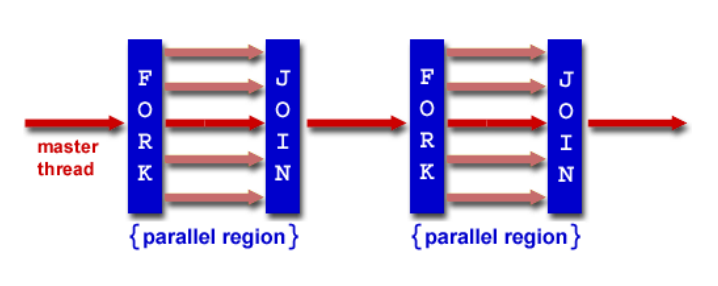
\includegraphics[width=0.6\textwidth]{images/forkjoin.png}
    \caption{Fork-Join Model}
    \label{fig:forkjoin}
\end{figure}
The program begins as a single thread called master thread. Then when it encounters parallel construct, it forks/spawns
a team of threads. The statement are then executed in parallel for the parallel region. At the end of the parallel region the team of threads synchronize and terminate and join
back to the master thread.

This is one of the good things about OpenMP has selective parallelism i.e. only certain sections of the code are executed in parallel based on the requirement. Thereby we are adhering to Amhadal's Law which says that not all parts of the code can be parallelized
and only certain parts of the code can be parallelized. Thus we are not spawning all of the program in parallel and only those where we require parallelism.

OpenMP consists of:
\begin{itemize}
\item Work-sharing constructs: specifies how region should be parallelised and distributed among threads.
\item Synchronization constructs: for providing synchronization between threads.
\item Data environment constructs: for specifying which data is shared and which is private.
\item Library calls, environment variables: special function calls and set environment variables. (set env command before executing your code).
\end{itemize}
A construct is a directive combined with the region where the directive applies. Above shown are the three constructs OpenMP supports.
OpenMP support loop-level parallelism to parallelize mainly for/do loops. If there are no dependencies between the iterations of the for loops then we can distribute this iterations to the processes
where some process executes some set of iterations and the other process executes the other set of iterations. This is called loop-level parallelism.
It gives the user a control over the fine-grained parallelism i.e.what regions to be parallelised. Hence, we call this as fine-level parallelism.
It follows Amdahl's law which says that only certain parts of the sequential code can be parallelized which is what is seen in this case. Note that in this we can also change the phases of parallelism meaning that 
based on the requirement we can change the number of threads that are executing the parallel region. Regions which can be more paralleized, one can have more number of threads. This is called dynamic parallelism.
In addition OpenMP also supports coarse-level parallelism i.e. parallelism where executing completely two different sections of code in parallel in addition to fine-level parallelism.
In the recent versions of OpenMP it also support executions on accelerators (GPUs), SIMD vectorizations (automatically updates a vector in parallel units) and task-core affinity.
The task-core affinity refers to the fact that the tasks can be explicitly mapped to a particular core. This can be helpful when we want to keep data which is highly related closer in order to save time.

\subsection{Parallel Construct}

omp parallel is the parallel construct in OpenMP. 
It is used to create a team of threads. The syntax is as follows:
\begin{lstlisting}
#pragma omp parallel
{
    /*parallel region*/
}
\end{lstlisting}
The parallel construct is followed by a block of code which is executed by all the threads in the team. 
The block of code is called the parallel region. So when a compiler encounters the pragma omp parallel construct it creates a team of 
threads and the subsequent region inside the block is then executed in parallel. Before the encounter with the omp parallel the compiler will execute the code in 
the sequential manner on a master thread. This is thus achieved by the parallel directive along with the block of code to be executed in parallel enclosed in curly braces which will be executed in parallel by a number of threads is 
called parallel construct.

How many number of threads? There are various ways to specify it, one can set an environment variable from command line set env omp numthreads=number of threads. 
Another way is to use the omp set numthreads(number of threads) function in the code. We can also specify the number of threads in clauses.
The following clauses can be used:
\begin{itemize}
\item if (condition): will execute in parallel if the condition is true.
\item num\_threads (n): will execute in parallel using n threads.
\item default (shared | none): specifies the default data scope for variables within a parallel region. Should the variables be shared or private among the threads.
\item private (list): specifies a list of variables that are private to each thread.
\item firstprivate(list): specifies a list of variables that are private to each thread and are initialized with the value of the variable outside the parallel region.
\item shared(list): specifies a list of variables that are shared among all the threads.
\item copyin(list): specifies a list of variables that are shared among all the threads and are initialized with the value of the variable outside the parallel region.
\item reduction(operator:list): specifies a list of variables that are private to each threads and which undergo changes by different threads. Then at the end of this parallel region all of these private variables are combined using the operator 
specified to give a value.
\item proc bind (master | close | spread): specifies the binding of the threads to the cores. How you want the task to be distributed to the cores. To the same core as the master thread or close to the master thread or spread.
\end{itemize}
Consider the code as shown  in the listing below which return the number of threads used in the parallel region. So say n threads were used then it would return n, n times each time when executed by one of the thread. 
\begin{lstlisting}
#include <omp.h>
int main()
{
    int nthreads;
    #pragma omp parallel
    {
        nthreads = omp_get_num_threads();
        printf("Number of threads = %d\n", nthreads);
    }
    return 0;
}
\end{lstlisting}
I encourage you to run these codes by simply copying and pasting it into your IDE and then execute them to see the results.

Consider another Hello World code as shown in the listing below.
\begin{lstlisting}
#include <omp.h>
int main()
{
    int nthreads,tid;
    #pragma omp parallel private(nthreads,tid){
        printf("Hello World\n");
    }
    return 0;
}
\end{lstlisting}
So some number of threads will be spawned and you will see the Hello World printed by each of the threads.

\subsection{Work sharing construct}
The work sharing construct is used to distribute the work among the threads.using the parallel construct we have spawned multiple threads.
Now to specify how to distribute the work among the threads we use work sharing construct.
There are three types of work sharing constructs - loops, sections, single.

\subsubsection{for-loop}
It is used for a for-loop or a do loop using pragma omp for (clause) as in the case of parallel construct.
The following clauses can be used :
\begin{itemize}
\item private (list)
\item firstprivate(list)
\item lastprivate(list): here the value of the variable in the list is equal to the value that is set by the last thread.
\item linear(list):
\item reduction(operator:list)
\item schedule([modifier[,modifier]:]kind[,chunksize]): To 
distribute the iterations among 
the threads, schedule clause specifies how 
we schedule the iterations of the loop among the different threads.
\item collapse(n): Useful for nested level parallelism. Say two for loops are nested and we want to parallelize both of them then we can use the collapse clause. In general only one of the 
for loop collapses but using collapse clause we can parallelise both of them by collapsing both the for loops. Say first for loop executes for 3 iterations and the second for loop executes for two iterations, Then
using collapse we can consider them as a total of six iterations in parallel across the threads. If we don't use the collapse clause only the outermost three iterations will be distributed among the threads.
\item ordered(n): In some cases we want threads to execute in order i.e. we want the threads managed by the first thread to be executed first and then the second thread and so on.
\item nowait: To tell the threads not to wait for each other at the end of for loop. By default all the threads will be waiting for each other for all the threads to finish executing the for loop.
\end{itemize}
For construct is the most commonly used and th most important construct in OpenMP.
Note that we are assuming that the iterations can be independently executed and simultaneously in parallel by the threads.
This works as long as the iterations are not dependent on each other whereas in the case when the iterations are dependent on each other say we are using a value in the loop which is dependent on the value resulted in previous loop,
in those cases the programmer should not use for construct.

Schedule clause: The assignment of iterations to threads depend on the schedule clause.
There are five schedule clauses. 
\begin{enumerate}
    \item schedule(static,chink size): In this the total number of iterations of the for loop will divided by this chunk size to obtain chunks and these chunks are distributed to the threads in a round-robin manner.
    For example, say 20 iterations of for loop and say chink size is 2 then 20/2 = 10 chunks are formed which each consisting of two iterations (first chunk consists of first two iterations and so on) and say we have only four threads then these chunks are distributed among these four threads in a round-robin manner.
    First chunk to first thread, second chunk to second thread, third chunk to third thread, fourth chunk to fourth thread and back from fifth chunk to first thread and so on.
    \item schedule(dynamic, chunksize): It is the same as above but here the chunks can be distributed dynamically, based on  OpenMP runtime system libraries own policy to distribute these chunks to the 
    threads that are ready to execute in a dynamic fashion.
    \item schedule(runtime): Here we give complete freedom to the OpenMP library to distribute the iterations based on the availability of thread.
\end{enumerate}

Consider the following for-loop example code \ref{lst:for-example}.
\begin{lstlisting}[caption={for-Example: Addition of two Arrays},captionpos=b,label={lst:for-example}]
#include<omp.h>
#define CHUNKSIZE 100
#define N 1000
main(){
    int i,chunk;
    float a[N],b[N],c[N];
    /*some initializations*/
    for (i=0;i<N;i++)
        a[i]=b[i]=i*1.0;
    
        chunk=CHUNKSIZE;
        #pragma omp parallel shared(a,b,c,chunk) private(i) {
            #pragma omp for schedule(dynamic,chunk) nowait
            for(i=0;i<N;i++)
            {
                c[i]=a[i]+b[i];
            }/*end of parallel section*/
        }
}
\end{lstlisting}

Here we ared adding two arrays a and b to form a third array c.
Note that we can perform this additions completely independent of each other and hence a good opportunity 
for using parallelism.
First for parallelization we need to spawn the threads for which we used pragma omp parallel shared(a,b,c,chunk) private(i).
Here a,b,c are shared among all the threads (since they could be very large arrays) and chunk is also a shared variable and iterator i is private variable to each thread because each thread is going to 
have its own set of iterations, and those set of iterations should be managed by a private iterator i to avoid any conflicts between which iterations to perform among the threads. 
Then we use the for construct to parallelize the for loop with a dynamic schedule clause and nowait for threads to not wait after finishing their iterations.
Note we can also combine the two pragma into one line in the code as pragma omp parallel for shared(a,b,c,chunk) private(i) schedule(dynamic,chunk) nowait.

\subsubsection{Coarse Level parallelism - Sections and Tasks}
In addition to fine-level parallelism as shown with the for loop example, OpenMP also supports coarse-level parallelism.
When we talk about given a set of iterations to a thread that is a fine-level parallelism regarding the iterations of the for loop.
but now suppose that we wish to execute two different functions containing many such for loops in parallel then it requires a coarse-level parallelism, we can use the sections construct.
Consider the following code showing use of sections construct as shown in the listing \ref{lst:sections}.
\begin{lstlisting}[caption={Sections Construct},captionpos=b,label={lst:sections}]
#pragma omp parllel sections <\clause-list\>
{
    #pragma omp section
        structure-block i
    #pragma omp section
        structure-block j
    ...
}
\end{lstlisting}
NOw suppose the structure blocks consists of functions and we wish to execute them in parallel, then as shown, we first enclose the entire in pragma omp sections and then 
the small parts which we wish to execute in parallel to be in pragma omp parallel section
Then the first section will be executed by one thread and the second section will be executed by another thread and so on.

OpenMP also supports dynamically spawning tasks. Suppose you have a parallel region and you wish to execute a few set of statements (a task) i.e. we are dynamically creating a task.
This generally occurs in large simulations where depending on the requirement one might need to create a task dynamically. This is done using the task construct. This task will be automatically assigned to one of the threads.
This is another coarse-level parallelism that OpenMP supports. Tasks is more dynamic construct where your code might be creating tasks dynamically and you want to assign them to the threads dynamically.
Task will be assigned to one of the threads you have spawned by OpenMP. You can also use a depend clause which allows us to create dependencies between the tasks by specifying 
certain variable\_list. Suppose a tasks uses some variable x and executes its program and now we wish to use that variable for another task such that the second task depends on the first task.
Then we can use the depend clause to specify that variable and thus to have the second task depends on the first task. This is done using the depend clause. Thus, it creates dependencies between variables and thus, second task
begins execution only after the first task has finished execution. Thus, it creates the dependencies between the tasks.
Now you can dynamically create task graphs where nodes in the graphs represent the tasks and the edges between the nodes represent the dependencies between the tasks.
This is a very powerful construct in OpenMP. Thus, with the tasks construct OpenMP can follow its own scheduling mechanism to assign the tasks to the threads such that the dependencies are maintained.
This is as shown in the listing \ref{lst:tasks}.
\begin{lstlisting}[caption={Tasks Construct},captionpos=b,label={lst:tasks}]
#pragma omp parallel \<clause-list\>
{
    ...
    #pragma omp task \<clause-list\>
    ...
    #pragma omp task depend(dependence type: variable\_list)
}
\end{lstlisting}

\subsection{Synchronization Directives}
Having distribute work among the threads there is always a chance of threads accessing some common variables. Hence, you need to synchronize the threads 
and protect certain variables using locking mechanisms.
OpenMP supports this using the following synchronization directives:
Note that all of this are already enclosed in a parallel region/parallel construct.
\begin{itemize}
    \item pragma omp master: This is used to specify that the block of code following this directive is executed by the master thread only.
    This is generally useful for print statements where you want only one thread to print the output. Say to print the value of a variable.
    \item pragma omp critical: This is used to specify that the block of code following this directive is executed by only one thread at a time.
    Say you are updating a variable and we do not want multiple threads to update the variable at the same time else it might result in garbage values.
    Then we can use the critical directive to protect the variable by enclosing that statement in this directive and only one thread can update the variable at a time.
    \item pragma omp barrier: This is used to specify that the threads wait at this point until all the threads have reached this point.
    \item pragma omp atomic: This is used to specify that the operation statement (expression) following this directive is executed atomically i.e. only one thread can execute this operation at a time.
    \item pragma omp ordered: This is used to specify that the block of code following this directive is executed in the order of the thread number. Say we want the first thread to execute those statements first and then the second thread to execute those statements and so on.
    This is useful when we want to maintain the order of the threads executing the statements.Say for example an array is distributed among threads and then we wish to print the entire array. Then we would like to print the array in the order of the threads i.e. the first set of elements residing in the first thread to print and then the second and so on.
    \item pragma omp flush: This is used to specify that the threads flush their private data to the shared memory. This is used to ensure that the shared memory is updated with the latest values of the private data.
    For example, say a thread has updated a variable and we want to ensure that the shared memory is updated with the latest value of the variable. Now there is no guarantee that the variable can be updated immediately to the shared array and be visible to the other threads. There may be a time lapse before it gets written to the shared array and before its visible to the other threads.
    Because the operating system maintains its own buffers where it may store the variables. Instead, if we wish to immediately flushed out so that it is visible to the other threads, then we can use the flush directive.
    Flush directive is used when we wish to see consistent vie of memory among the threads. Using flush directive, Thread-visible variables (global variables, shared variables etc..) are written to memory. If a variable list is used, only variables in the list are flushed.
    Consider the following code as shown in the listing \ref{lst:flush}.
\begin{lstlisting}[caption={Flush Directive},captionpos=b,label={lst:flush}]
int sync(NUMBER_OF_THREDS);
float work[NUMBER_OF_THREADS];
#pragma omp parallel pritvate(iam,neighbor) shared (work,sync)
{
iam = omp_get_thread_num();
sync[iam]=0;
#pragma omp barrier

/*Do computation into my portion of work array*/
work[iam]=compute(iam);

/* Announce that I am done with my work
    * The first flush ensures that my work is
    * made visible before sync.
    * The second flush ensures that sync is made visible.
*/
#pragma omp flush(work)
sync[iam]=1;
#pragma omp flush(sync)

/* Wait for neighbor*/
neighbor = (iam>0?iam : omp_get_num+threads())-1;
while(sync[neighbor]==0){
    #pragma omp flush(sync)
}
/* Read neighbor's values of work array*/
...=work[neighbor];
}
\end{lstlisting}
    Here in the example, a thread writes its respective value to its respective array elements and at the same time 
    neighboring thread tries to read the values that are written by this particular thread. Since, the neighboring threads are trying to read the values that are written by the threads, we need to ensure that the values are written to the shared memory before they are read by the neighboring threads.
    This is done using the flush directive. The first flush directive ensures that the values are written to the shared memory before they are read by the neighboring threads. The second flush directive ensures that the sync array is made visible to the neighboring threads.
    The above shown SPMD code is executed by all the threads. From the perspective of a thread the iam variables denotes its thread id, the neighbor represents the neighboring thread id. The 
    work and sync are the variables that are shared among the threads. The work array is the main array where the threads write their respective values (and also being read by the other threads) and the sync array is used to signal the other threads to say that this thread has finished writing to the work array
    so that the other thread can read those values. In order to ensure that the values are written to the shared memory before they are read by the neighboring threads, the sync variable has to be flushed out.
    Note that we can get the thread id as shown in the code using omp\_get\_thread\_num. So at the beginning of the code each thread will get its thread id and then set the sync[id]=0 and then barrier is used to ensure that all the threads have reached this point.
    Each thread then does some computation and at the end of the computation stores its result to its corresponding work element. Now it requires to announce that it is done with its work so that the neighboring thread can make use of that value.
    This is done using flush statement so that the changes in work array is visible and then it changes the value of sync array to 1 to signal the other threads that is is done. Then another flush statement so that the changes in sync are visible.
    Then the neighboring threads will find out its thread id based on their own thread id and will actively look whether the neighboring variables are updated or not. If not then it will keep on checking until the neighboring thread has updated the value  (because of the while loop),
    it keeps flushing the sync variable. Once the sync variable is updated then it reads the value of the work array of the neighboring thread.
\end{itemize}

\subsection{Data Scope Attribute Clauses}
OpenMP supports many clauses supporting data scope. Data scopes is explicitly specified by data scope attribute clauses.

\begin{enumerate}
    \item private: A separate variable will be created fore each of the thread and it is initialized to the default value to which any programming language initializes it to( generally garbage values by default in C/C++).
    \item firstprivate:  If you want a private variable for a thread to be initialized with value of the variable that existed before entering the parallel clause i.e. value in the master thread, it is to be declared as firstprivate. In this, separate private copies will be created for each thread and the value will be initialized to that of a variable in the master thread before entering the parallel region.
    \item lastprivate: When you exit a parallel region the value that will be assigned to the variable will be the one that is assigned by the thread that executed at last. In a parallel region, multiple threads will be executing, the value of this private variable will be the one assigned by the thread that executes at last to the variable in the master thread.
    \item shared: Declaring the list of variables to be shared among the threads.
    \item default: To set the default behavior of the variables in the parallel region. Most variables are shared by default.
    \item reduction: If you wish to combine all the private variables in all the threads and reduce it using some operator (say like addition) to get the final value of the reduction to be assigned to a variable in the master thread after exiting the parallel region.
    \item copyin: Copyin acts similar to private.
    \item copyprivate: It is used to assign thread private variables and if you wish to assign some variables as thread private and initialize them, then we use copyprivate. More will be seen later.
\end{enumerate}
Sometimes while declaring a large multidimensional arrays as private leads to overhead because now each thread would have to create this large multidimensional arrays. Moreover, declaring them as firstprivate will incur even further overhead as each thread now also requires it to initialize the threads which results in overheads.

\subsubsection{threadprivate}
They are global variable-list where private copies are maintained for each thread (just like private variables) but the variable values will exist across different parallel regions. Say for example say a variable x is declared as threadprivate, then separate copy of x will be maintained for each of the threads. Say now at the end of the first parallel region the value of the variable x in the first thread is say 5. Now in the next parallel region if we declare the variable x as private then the value of 5 will be lost and x will be initialized to some other initial value in the first thread. This would happen if we had not declared the variable x as threadprivate. But since we have declared the variable as threadprivate, the value 5 will exist across multiple parallel regions in the first thread. So for doing this, we declare a variable using a special directive threadprivate instead of private. Consider the following code \ref{lst:threadprivate}.
\begin{lstlisting}[caption={threadprivate Directive},captionpos=b,label={lst:threadprivate}]
#include<omp.h>
int alpha[10], beta[10], i;
#pragma omp threadprivate(alpha)
main(){
    /* explicitly turn off dynamic threads*/
    omp_set_dynamic(0);
    /*First parallel region*/
    #pragma omp parallel private(i,beta)
    for(i=0;i<10;i++) alpha[i]=beta[i]=i;
    /*Second parallel region*/
    #pragma omp parallel
    printf("alpha[3]=%d and beta=%d\n",alpha[3],beta[3]);
}
\end{lstlisting}
Note that we have declared alpha as threadprivate variable.
In the first parallel region we have declared i and beta as private variables to each thread.  Then in the first parallel region we are assigning value to alpha and beta arrays equal to their array index i (alpha is threadprivate and beta is private).
Then in the second region when we print the value of alpha[3] we will get a value of 3 since alpha has been declared as a threadprivate variable and hence will maintain its value across different parallel regions. But when we print beta[3] we will get some garbage value (or may be some initial value if initialized in the second parallel region). This is because we have declared beta as private and not threadprivate. So for beta its scope exists only inside that parallel region whereas for alpha its scope exists across different parallel regions. Hence, if we want the scope of a variable to span across different parallel regions we have to declare them as threadprivate. Note that here the parallelism should be the same for using threadprivate i.e. say if you have spawned 4 threads in the first parallel region then you must spawn only 4 threads in the next parallel region. Thus, we have used set\_dynamic(0) to turn off the dynamic parallelism. If we leave it to OpenMP then it may spawn different number of threads in different parallel regions.

\subsubsection{default-example}
Consider the following example code for better understanding of concepts of private, shared and default \ref{lst:default}.
\begin{lstlisting}[caption={default-Example},captionpos=b,label={lst:default}]
int x, y, z[1000];
#pragma omp threadprivate(x)

void fun(int a){
    const int c = 1;
    int i = 0;

    #pragma omp parallel default(none) private(a) shared(z)
    {
        int j = omp_get_num_thread();
            //O.K. - j is declared within parallel region
            a = z[j];
            x=c;
            z[1]=y;
    }
}
\end{lstlisting}
Here we have declared variables x, y and array z as global variables. In this code we have declared x as threadprivate variable.  We have a function fun in which we have declared a const it c and int i. Then in the clauses while entering the parallel region we have declared default as none which means that we do not want any of the variables to be shared by default. Then we have declared variable a as private to each of the thread and array z as shared among the threads. Inside the parallel region we have declared a variable j, this works since we have declared j locally to each of the threads. Then we do a=z[j], this works since a is listed as private and z is listed as shared. then we do x=c, this should also work since we have declared x as threadprivate and c is const-qualified type. Then we do z[i]=y, this will not work since although z is a shared variable, but variables i and y are not known inside the parallel region since by default we have set none thus, variables won't be shared inside the parallel region. Also, see that we have not declared anything about the variables y and i so they don't exist inside the parallel region (as default is set to none, if the default had been set to shared then the variables would have been shared and thus statement would have worked), thus compiler will flag this as error as cannot reference i or y here.

\subsection{Library Routines (API)}
In addition to the above seen Directive and clauses, OpenMP also supports certain functions like:
\begin{itemize}
    \item Querying function (number of threads etc)
    \item General purpose locking routines
    \item Setting Execution environment (dynamic threads, nested parallelism etc.)
\end{itemize}
Example of some of the functions are as follows:
\begin{itemize}
    \item OMP\_SET\_NUM\_THREADS(num\_threads): To set the number of threads you wish to spawn in the corresponding parallel region.
    \item OMP\_GET\_NUM\_THREADS(): To find the number of threads used in the parallel region.
    \item OMP\_GET\_MAX\_THREADS(): To query the maximum number of available threads you can get for a parallel region.
    \item OMP\_GET\_THREAD\_NUM(): To get the thread id of a thread inside the parallel region.
    \item OMP\_GET\_NUM\_PROCS(): To get the number of processors on which OpenMP is executing on.
    \item OMP\_IN\_PARALLEL(): To query whether you are in a parallel region.
    \item OMP\_SET\_DYNAMIC(dynamic\_threads): Set the number of threads to be spawned dynamically (chosen by OpenMP) or a certain value (say maximum) inside the parallel region.
    \item OMP\_GET\_DYNAMIC: 
    \item OMP\_SET\_NESTED(nested): To run on or off nested parallelism in OpenMP
    \item OMP\_SET\_NESTED()
    \item omp\_init\_lock(omp\_lock\_t *lock): To initialize a lock
    \item omp\_init\_nest\_lock(omp\_nest\_lock\_t *lock)
    \item omp\_destroy\_lock(omp\_lock\_t *lock): To free the lock
    \item omp\_destroy\_nest\_lock(omp\_nest\_lock\_t *lock)
    \item omp\_set\_lock(omp\_lock\_t *lock): For acquiring a lock
    \item omp\_set\_nest\_lock(omp\_nest\_lock\_t *lock)
    \item omp\_unset\_lock(omp\_lock\_t *lock): For releasing the lock
    \item omp\_unset\_nest\_lock(omp\_nest\_lock\_t *lock)
    \item omp\_test\_lock(omp\_lock\_t *lock): To see if the lock is available or not
    \item omp\_test\_nest\_lock(omp\_nest\_lock\_t *lock)
    \item omp\_get\_wtime(): To get the time taken in the parallel region by subtracting the time at the start and at the end of the parallel region.
    \item omp\_get\_wtick()
    \item omp\_get\_thread\_num(): Number of threads being used
    \item omp\_get\_num\_proc(): Number of processors you are currently using
\end{itemize}

\subsection{Locks}
OpenMP supports both simple locks and nestable locks. For a simple lock, if the thread acquires the lock once then it cannot acquire that lock once again i.e. you cannot use the set\_lock function twice for locking on the same variable by the same thread Thus, we cannot use a nest statement for locking simple locks. This will be a deadlock situation since the thread that once who has acquired lock on it and now putting a lock again means it will be waiting for it to be released but since it was the one to acquire it it will be waiting forever to acquire it once again since the lock will never be released. A lock can be released only by the thread that acquires it. So till the thread does not release the lock it cannot acquire it once again. So acquiring the lock twice in a row will lead to a deadlock situation.

In some cases, it may be desired to use a nested lock. For example in case of some Linear Algebra libraries using OpenMP functions and there are say multiple routes from the main function to enter into those functions. Say there are multiple ways of accessing those functions. then it is desired to protect each of the functions and thus use nested locks.

Simple locks are not locked if they are already in a locked state. nestable locks can be locked multiple times by the same thread. Simple locks are available if they are locked. Nestable locks are available if they are unlocked or owned by a calling thread i.e. it uses a counter to count the number of locks on it by different threads and they will be released based on the same manner they were locked by different threads in their calling manner, thus they need to be released by all other calling threads for a thread that wishes to use it.

Consider the following code to show the importance of nested locks \ref{lst:nested}.
\begin{lstlisting}[caption={Nested lock-Example},captionpos=b,label={lst:nested}]
#include<omp.h>
typedef struct {int a,b; omp_nest_lock_t lck;} pair;

void incr_a(pair *p, int a)
{
    // Called only from incr_pair, no need to lock.
    p->a +=a;
}
void incr_b(pair *p, int b)
{
    //Called both from incr_pair and elsewhere,
    //so need a nestable lock.

    omp_set_nest_lock(&p->lck);
    p->b+=b;
    omp_unset_nest_lock(&p->lck);
}
\end{lstlisting}
In the above code we have declared a structure which has two integer variables a and b and a lock. pair is a variable of struct type. There are two function declared as incr\_a and incr\_b. Consider that incr\_a is called only from incr\_pair so there is no need for lock. Now consider the function incr\_b which is say called from both incr\_pair and elsewhere, thus we need a nestable lock in order to avoid simultaneous updation (or else may lead to garbage values). Thus we have used set and unset lock around it.

Now consider the following continuation of the code as shown in \ref{lst:nested2}.
\begin{lstlisting}[caption={Nest lock-Example2},captionpos=b,label={lst:nested2}]
void incr_pair(pair *p, int a, int b)
{
    omp_set_nest_lock(&p->lck);
    incr_a(p,a);
    incr_b(p,b);
    omp_unset_nest_lock(&p->lck);
}
void f(pair *p)
{
extern int work1(), work2(), work3(0;
#pragma omp parallel sections
{
    #pragma omp section
        incr_pair(p,work1(),work2());
    #pragma omp section
        incr_b(p,work3());
}
}
\end{lstlisting}
In this example note that we are using parallel sections for calling the funtions incr\_pair and incr\_b, and each of those functions act on p.  Now note that incr\_a is called only from incr\_pair and thus there is no need for lock, but note that incr\_b is called from incr\_pair as well as directly from incr\_b. Thus, it requires a nested lock for locking the value of p while performing the operation and then releasing the lock, which is done by incr\_pair and incr\_b using set and unset lock functions.


\subsection{Example 1: Jacobi Solver}
This is an example of previously explained grid solver, excpet for the fact that here we are parallelizing across the iterations and not across the rows. Consider the following code as shown in \ref{lst:jacobi}
\begin{lstlisting}[caption={jacobi-solver},captionpos=b,label={lst:jacobi}]
#include<omp.h>
int main(int argc,char**argv){
...
int rows,cols;
int* grid;
int chunk_size, threads=16;
...
    /*Allocate and initialize the grid */
    grid=malloc (sizeof(int*)*N*N);
    for(i=0;i<N;i++){
        for(j=0;j<N;j++){
        grid[i*cols+j]=...;
        }
    }

    chunk_size=N/threads;
    #pragma omp parallel for num_threads(16) private(i,j) shared(rows,cols,grid) schedule(static,chunk_size) collapse(2)
    for(i=1;i<rows-1;i++){
        for(j=1;j<cols-1;j++){
            grid[i*N+j]=1/4*(grid[i*N+j-1\+grid[i*N+j+1]+grid[(i-1)*N+j]+grid[(i+1)*N+j]);
        }
    }
}
\end{lstlisting}
So as can be seen in the code we have first initialized and then we have used a schedule in parallelizing the code.
For that we have declared the chunk\_size=N/num\_threads which is the total number of rows/columns divided by the number of threads=16. So in the next statement where we start parallel region using pragma omp parallel for indicates that we are using 16 threads, the iterators i and j have been declared as private. The number of rows, columns and grids are shared variables i.e. shared among threads. Then we are using static in the schedule clause so the total number of iterations will be given based on chunk\_size to each of the threads in a round robin manner. Note that we are also using collapse(2) which means that it will collapse the two for loops i.e. the total number of iterations will be considered as rows*cols and these many iterations will be distributed among all the threads based on the chunk\_size. In this if we had not used collapse then only the first for loop i.e. the iterations for the rows would have been distributed among the threads and now each thread would have to take care of all the iterations for the columns.

\subsection{Breadth First Search (BFS) Algorithm}
The idea behind BFS is that we start from some source vertex at level 0 and then in the first level we explore all the neighbours of the source vertex, then in the second level we pick one of the neighbours of the source vertex and explore its neighbours and so on till all the neighbours have been explored. Below shown is the parallel version of BFS.
\subsubsection{Version 1 (Nested Parallelism)}
Consider the following example code \ref{lst:bfsv1}
\begin{lstlisting}[caption={BFS-Example},captionpos=b,label={lst:bfsv1}]
...
    level[0] = s;
    curLevel = 0;
    dist[s]=0; dist[v!=s]=-1;

    while(level[curLevel]!=NULL){
    #pragma omp parallel for ...
        for(i=0;i<length(level[curLevel]); i++){
            v=level[curLevel][i];
            neigh=neighbors(v);

        # pragma omp parallel for ...
            for(j=0;j<length(neigh);j++){
            w=neigh[j];
            if(dist[w] = -1){
                level[curLevel +1]= union(level[curLevel+1],w);
                dist[w] =dist[v]+1
            }
            }
        }
    }
    
\end{lstlisting}
Here we are at first assigning only the source so the 0th level has only the source vertex s. The current level =0, and distance of the source vertex from the source vertex is set 0 and the distance of other vertex from the source vertex is set to -1. We are suppose to find the distance of the other vertices from the source vertex. 
Inside the while loop we keep on going until we don't see any nodes in the current level. Using the for loop we explore the vertices at the current level and check all its neighbours and store the neighbours in the variable neigh. Then in the next for loop we start at one of the neighbours and check if the distance is -1 i.e. whether it ha been already explored or not. If it has not been explored then we add that vertex into the next level and add the distance of that node as the distance till previous node +1. Thus, using two pragma omp for we are parallelizing both the for loops nesting the inner and outer for loops, thus a nested for parallelism.

In order to explain in further depth, what we have done is that we spawn a thread corresponding to each of the vertex in the current level which is done by the pragma omp for on the outer loop. Then for each of the vertex we further spawn threads for exploring its neighbours and adding the corresponding distance which can be done independently. Thus we are spawning threads inside a thread i.e. nested level parallelism.

\subsubsection{Version 2 (Task constructs)}
Here we are going to use task construct to implement the BFS algorithm.
Consider the following code \ref{lst:bfsv2}.
\begin{lstlisting}[caption={BFS-Example},captionpos=b,label={lst:bfsv2}]
...
    level[0] = s;
    curLevel = 0;
    dist[s]=0; dist[v!=s]=-1;

    while(level[curLevel]!=NULL){
    #pragma omp parallel ...
        for(v in level[curLevel]){
            for (w in neighbours(v)){
                # pragma omp task...
                {
                    if (dist[w]=-1){
                        level[curLevel+1]=union(level[curLevel+1],w)
                        ..
                        dist[w]=dist[v]+1;
                    }
                }
            }       
        }   
    }
\end{lstlisting}
Here we are not using for construct instead we are just opening a parallel region and anytime we are required to process a neighbour then for that neighbour we are dynamically creating a task, the task will be dynamically assigned to OpenMP threads by the OpenMP library.

\newpage

\section{Message Passing Interface - MPI}
Recall that MPI uses distributed memory parallelism. Here we have explicit communication and synchronization. Thus, unlike in the case of shared memory paralellism where we just used parallel constructs in order to make the program work in parallel, here, we will be required to write an explicit program to be run by each of the processors. Hence, MPI is said to have high programming complexity. MPI is highly popular because even though you may have high multiple cores within a node, for very large problem you need to have many such nodes and when you have many such nodes the only way to share information between parallel processes executing on these two nodes is through message passing and hence we have to inevitably used MPI for it.

\subsection{MPI Intrdocution}
It is a stanard for explicit message passing in MIMD machines. Thus, a MPI program on one machine will also work on any other machines. Thus, it supports portability, and is a standard for hardware vendors. Currently the latest version is MPI-3 in 2012.
MPI containes the following standards:
\begin{itemize}
    \item Point-Point: point to point communications. When we are required to send information from one process to another process using a send and receive function.
    \item Collectives: When we wish to communicate across multiple processes, they are done using this collectives.
    \item Communication contests: For each communication it defines a scope.
    \item Process topologies: MPI supports process topologies. Recall that we have already seen network topologies. Network topologies refer to how the processes are connected as a mesh, bus, star, etc..
    All these happen at the hardware level. Likewise at the programming level the processes may have certain communication pattern. Example, may be in a linear manner or in a mesh like manner. This is called Process topologies.
    \item Profiling interface: MPI allows profiling interface that is to implement MPI functions so that you can create a library of your own.
    \item I/O: This is defined in MPI standard 2. How can we make multiples processes read and write data simultaneously.
    \item Dynamic Process groups: MPI -2 allows you to dynamically spawn multiple processes during the execution.
    \item One-sided communication: Like in Shared memory parallelism where only one process is required for communication. Here, in MPI 2 using one-sided communication can be used where one of the process just adds data and there is no other process required to receive that data. Thus, instead of requiring two processes to share data we can have only one process which can put data into a remote process memory without requiring the other process to receive it.
    \item Extended collectives:
\end{itemize}
There are many such MPI functions which can be used to write a program. 

\subsection{Communication Primitives}
\subsubsection{Point-Point Communications}
\begin{lstlisting}
MPI_SEND(buf,count,datatype,dest,tag,comm)
MPI_RECV(buf,count,datatype,source,tag,comm,status)
MPI_GET_COUNT(status,datatype,count)
\end{lstlisting}
Here, sending data from one process to another is called MPI\_SEND.
The sending process will send an array, along with the count of number of elements in that array, and the data type of the array elements. 
The buf, count, datatype corresponds to MPI message i.e. the sender process that wants to send message is defined by these three parameters to another process called the reciever process. 
\begin{itemize}
    \item dest: To identify the receiver process the sender process should give the id of the receiver process. In MPI terminology. we call these ids as Rank of a process. When we spawn a set of process, each process will get a rank starting from 0 to p-1, where p is the number of processes. For example, if process 0 wishes to send a message to process 4, the it will fill 3 in the dest.
    \item tag: Just like the identifies for the process, it also gives identifier for the message. This is especially useful when a sender process wants to send multiple messages to the same reciever process and we want the receiver process to demarcate the messages clearly, then we need to use message id.
    \item comm: It shares the communication context. It is a communicator pointer available to the process that calls this function the pointer points to a communication group 
\end{itemize}

Similarly, for MPI\_RECV:
\begin{itemize}
    \item buf: When the message is send it will be received in this as the receiving buffer.
    \item count: This will count the number of elements in the array that is supposed to be receive.
    \item datatype: The datatype of the received data.
    \item source: Just like sender has to say for which process it is sending to, the receiver has to mention from which process it is receiving from which is by giving the rank of the process it is receiving from.
    \item tag: It also needs the same tag as that of the sender process so that the message is matched with the receiver process
    \item comm: Then a communicator.
    \item status: It is an extra parameter to find out the status of the message. For this we can use MPI\_GET\_COUNT(status, datatype,count) to know how much of the data you ended up receiving.
\end{itemize}

When you initially start a process all the processes will belong to a certain group and all the processes will be given a rank with respect o processes in the group. In MPI you can create subgroups (may or may not be overlapping). Inside a subgroup the process can have different ranks with respect to other processes in the sub group than the ones originally assigned. For example, withing a group say a process is ranked 4, then in a subgroup consisting of that processor it can be ranked 0. Thus, the process had id 4 with respect to overall group but now has rank 0 with respect to its subgroup. Thus a particular process can have multiple ranks depending upon the subgroup you are considering it in. Thus, say that sending to rank r is now confusing since there could be multiple processes with rank r within different subgroups, thus, we need to also mention the subgroup, only then the process you are sending to it will be clear.  Thus, we not only need to tell the rank but also the communication scope/communication group with which you are referring . That communication group is pointed to by a variable called the communicator.

Consider the following simple example code
\begin{lstlisting}
comm=MPI_COMM_WORLD
rank=MPI_Comm_rank(comm,&rank);
for(i=0;i<n;i++) a[i]=0;
if(rank==0){
    MPI_SEND(a+n/2,n/2,MPI_INT,1,tag,comm);
}
else{
    MPI_RECV(b,n/2,MPI_INT,0,tag,comm,&status);
}
/*process array a*/

/*do reverse communication*/
\end{lstlisting}
Let us assume only two processes in the overall world with no subgroups. The overall group in MPI is called by a default value MPI\_COMM\_WORLD.
MPI\_Comm\_rank is a special utility function to find out the rank with respect to the particular group that you are belonging to. The above shown is a SPMD program. Thus when the program is executed by the process it will get its own id/rank in the overall group stored in the variable rank. MPI\_INT are called wild cards which is used to define integers, similarly, MPI\_DOUBLE stands for double and so on. Now in thcode we initialise an array and then the process whose rank=0 send the second half of the array to the process with rank=1. See that we we are sending A=n/2 in the buff and then n/2 elements of the array whose datatype is integer. We can use some integer value (say 5) as tag/id of the message, then the comm refers to the process 1 in the overall communicator defined in the MPI\_COMM\_WORLD. In the else loop, the process whose rank is not zero i.e. rank 1 will do MPI\_RECV and will receive the message into its array and will receive n/2 elements of the array of data type int (MPI\_INT) from process 0, with the same tag and comm, and the status stored in the variable by \&status. After that the processes work on their individual arrays in parallel.

The default communicator is MPI\_COMM\_WORLD which includes all processes We can also use Wild cards in the MPI\_RECV function in the receiver source and tag fields as MPI\_ANY\_SOURCE and MPI\_ANY\_TAG respectively. This is extremely useful when a particular process is receiving messages, using this, it does not need to worry about any particular order in which it should receive and it could receive in any order if we use MPI\_ANY\_SOURCE. Likewise MPI\_ANY\_TAG can be used when a particular process is receiving multiple message from multiple sources with multiple message ids and the if the order of messages does not matter, then, in that case we can specify wild card MPI\_ANY\_TAG. Recall that we can also use MPI\_COMM\_RANK to get the process rank/id.

Following are a few Utility functions in MPI:
\begin{itemize}
    \item MPI\_INIT: This is used to initialize the MPI environment at the beginning of the program.
    \item MPI\_FINALIZE: This is used to finalize the MPI environment at the end of the program.
    \item MPI\_Comm\_size(comm,\&size): With the function a process can find out how many processes are involved in the MPI communicator world that you enter (here comm).
    \item MPI\_Comm\_rank: A process can query its own id.
    \item MPI\_Wtime(): It is used to get the time spent in the parallel region of the code by inserting before and after the section and then subtracting to get the time taken in that section of the code.
\end{itemize}

\subsubsection{EXAMPLE 1: Finding maximum using 2 processes}
Consider the following C program.
\begin{lstlisting}
#include "mpi.h"
int main(int argc,char** argv){
    int n;
    int* A, *local_array;
    int max, local_max,rank1_max,i;
    MPI_COMM comm;
    MPI_Status status;
    int rank, size;
    int LARGE_NEGATIVE_NUMBER=-999999;
    MPI_Init(&argc,&argv);

    comm=MPI_COMM_WORLD;
    MPI_Comm_size(comm,&size);
    MPI_Comm_rank(comm,&rank);

    if(size!=2){
        printf("This program works with only two prodcesses.\n");
        exit(0);
    }
    if(rank==0){
        /*Read N from console*/
        MPI_Send(&N,1,MPI_INT,1,5,comm);
        /*Do dynamic allocation of A array with N elements*/
        /*Initialize an array A of N elements*/
        /*Do dynamic allocation of local_array with N/2 elements */
        for(i=0;i<N/2;i++){
            local_array[i]=A[i];
        }
        MPI_Send(A+N/2,N/2,MPI_INT,1,10,comm);
    }
    else{
        MPI_Recv(&N,1,MPI_INT,0,5,comm,&status);
        /*Do dynamic allocation of local_array with N/w elements */
        MPI_Recv(local_array,N/2,MPI_INT,0,10,comm,&status);
    }
    local_max=LARGE_NEGATIVE_NUMBER;
    for(i=0;i<N/2;i++){
        if(local_array[i]>local_max){
            local_max=local_array[i];
        }
    }

    if(rank==1){
    MPI_Send(&local_max,1,MPI_INT,0,15,comm);
    }
    else{
        max=local_max;
        MPI_Recv(&rank1_max,1,MPI_INT,1,15,comm);
        if(rank1_max>max){
            max=rank1_max;
        }
    }
    printf("Maximum number is %d\n",max);

    MPI_FINALIZE();
}
\end{lstlisting}
This program tries to find out maximum element in an array using two processes. Note that we need to include mpi.h header file to use MPI. Then we declared a communicator comm of type MPI\_Comm. Then another variable status of type MPI\_Status which will be used in receive function. We first initialize the MPI environment using MPI\_Init and pass the arguments \&argc,\&argv. Then we use the default communicator MPI\_COMM\_WORLD and store it in comm variable. Then using MPI\_Comm\_size we can find the total number of processes with which this program is started and then find its own ran using MPI\_Comm\_rank.
Since the program is required to use only two processes we put a check on the number of processes with which user starts using if loop. If the size is not equal to it prints the statement or else we continue with the algorithm. If rank =0 for the process, it will read N from the console and then sends that N to the Processor with rank 1. This is done using the MPI\_Send command with sending the address using \&N and since its only 1 value we write 1 in place of count, since the datatype of N is an integer we write MPI\_INT. If the process is not rank=0 i.e. rank=1, it will receive similarly using MPI\_Recv as shown in the code above. Then the process 0 dynamically allocates the array A with N elements and initializes it. The process 0 then reads the first half of the array and stores it in its local array. It then sends the second half using MPI\_Send to the process with rank=1. Note that in this case we used message id as 10. Then the process with rank=1 receives it into its local array. 
Then after storing the value of large negative number in local\_max, we use a for loop which is executed by both the processes to find the maximum in their own part of array. This is a case of SPMD program where the same program is executed by multiple processes on different data. Both then find the local maximum and then the process with rank=1 sends its maximum to process with rank 0 and after process with rank 0 compares both the maximum and chooses the larger one and prints the maximum number. Then we use MPI\_Finalize to end the MPI environment.

\subsection{Buffering and Safety}
One of the important aspects related to send and receive is send and receive buffers. In order to understand this better consider an example. Say you have a written a program and in it you call MPI\_Send(user\_buf,...) where user\_buf refers to the buffer (data address) to be send. This user program is linked with a MPI library. So when user program uses MPI\_Send it calls the MPI library which implements the MPI functions and interacts with the underlying hardware and network using TCPIP protocols (Tcp\_send()) in the networks functionality, which will then be received by some receiver. At the receiver side there is a MPI library which has implemented MPI\_Recv using the underlying network receive. This is then called by the receiving process in the user program by invoking the function MPI\_Recv. The MPI libraries will have its own global send and receive buffer, and at some point in the MPI library implementation of MPI\_Send the user\_buf gets copied into the send\_buf and likewise after the message is received in the MPI library inside the MPI\_Recv function it gets copied from recv\_buf to user\_buf. MPI\_Send also spawns threads and then return. This threads take care of any additional overhead like inserting message headers, dealing with acknowledgments and invoking the network send function TCP\_send(). The user program does not have to wait for all of these since inside the MPI library function it spawns threads to take care of the sending and then immediately returns because the main thread which called this function can immediately return and make progress with the subsequent statements. Behind the scenes, MPI library threads is still taking care of sending the communication. Likewise is the case with MPI recv\_buffer. This is called blocking send and blocking receive because the MPI\_Send has to wait till the user\_buf gets copied into send\_buf. Likewise MPI\_Recv has to block or wait until the message from recv\_buf is safely copied to user\_buf passed by the receiving function.

Consider the following three scenarios.
Case 1: Process 0 does MPI\_Send and then MPI\_Recv and the process 1 does the matching receive MPI\_Recv and then a matching send MPI\_Send for the receive in process 0. This kind of program always works since it has simply the send corresponding to a receive and a receive corresponding to a send. 

Case 2: Now consider a scenario where process 0 does MPI\_Recv and MPI\_Send and process 1 does MPI\_Recv and MPI\_Send. Now the process 0 can make progress only after it has received from process 1 and similarly process 1 can proceed only after it receives from process 0. Thus, unless both the processes do not receive they cannot proceed to their next statement of MPI\_Send which is the corresponding statement for the other process. So both of them cannot proceed and will be waiting for each other. Hence, this situation will result in a deadlock.

Case 3: Now consider a situation where Process 0 first calls MPI\_Send and then MPI\_Recv and the process 1 does MPI\_Send and then MPI\_Recv.
This will work because the process 0 user buffer that is passed in the MPI\_Send will be safely copied to MPI implementations send\_buf and will return to the user program. While the communication is happening in the background threads, the process 0 will call MPI\_Recv function. At the same time process 1 calls MPI\_Send and the corresponding MPI\_Recv function in process 0 will be able to receive it. Hence, there is a progress in the program as in the process 0 we will safely return from MPI\_Send operation since the user\_buf was safely copied to send\_buf and the function returns and continue on to the next statement in the user program to receive from process 1. Likewise process 1 will be able to execute MPI\_Recv statement. This may or may not work provided that the MPI libraries send and receive buffers have got sufficient space to accommodate the message that is being passed in the user\-buf. This is because send\_buf is an internal buffer that is maintained by the MPI library and it cannot allocate really large size buffers because if it allocates large size buffers a significant amount of memory will be consumed by the MPI library and there will be very little memory left for the user program for its own variables. So MPI implementation have typically fixed size buffers. If the fixed size buffer is of adequate capacity greater than message size being sent using MPI\_Send then it will work as described and user\_buf will be safely copied to send\_buf and it will then safely proceed. On the other hand, if the implementation buffer send\_buf is smaller in size than the user\_buf passed in MPI send then all the part of the user\_buf will not copied and only some part of it will be copied and thus in order to send all of the message, the copied part needs to be send first and received by the receiving process and then when the buffer is empty and the entire message is again copied and this process goes on. But note that in order for the buffer to copy the entire message it needs to first send the already copied part to the required processor which then needs to be received by the receiving end processor. If the receiving end processor is also trying to send as in this case then the situation will lead to a deadlock situation, as both the processes are not waiting for the other process to start receiving so that the rest of the user\_buf can be copied to the send\_buf. Overall, if the implementation buffer is of adequate capacity then this work or else if it is of a lesser capacity than the user\_buf then it will result in a deadlock situation. Note that this is not the case with case 2 because here the implementation will require the MPI\_Recv to first receive all of the message before moving on to the next statement. Thus case3 may or may not work and hence is an unsafe way of writing program so avoid writing those kinds of programs.












    









\newpage

%For references to the notes
\begin{thebibliography}{9}
    \bibitem{parallelcomputingtutorial} 
    \weblink{http://www.llnl.gov/computing/tutorials/parallel_comp/}{Parallel Computing Tutorial} - Reference for Introduction, Classification of Architectures - Flynn's Taxonomy, and Classification based on Memory.
    \bibitem{MathewJacobLecs}
    \weblink{https://youtu.be/-yMWgtTeQgY?si=_PIhzFH7zZTydzcM}{Mathew Jacob - Parallel Architecture Lectures} - Lecture 38 and Lecture 39 - Reference for Introduction, Classification of Architectures - Flynn's Taxonomy,and Classification based on Memory.
    %Insert a book reference
    \bibitem{AnnanthaGramaIntro}
    Section 2.4 from Kumar, V., Grama, A., Gupta, A., Karypis, G. (1994). Introduction to parallel computing (Vol. 110). Redwood City, CA: Benjamin/Cummings for Network Topology, Shared Memory Architecture and Cache Coherence Protocols.
    %INsert Other readings
    \bibitem{NVIDIAGoogleA100}
    Many-core - Google for NVIDIA A100 white paper
    \bibitem{CullerandSingh}
    Section 2.2 and 2.3 - Culler, D., Singh, J. P., Gupta, A. (1998). Parallel computer architecture: a hardware/software approach. Elsevier.
    \bibitem{hpctutOpenMP}
    \weblink{https://hpc-tutorials.llnl.gov/openmp/}{OpenMP tutorial} - OpenMP tutorial for parallel programming.
    \bibitem{IntelOpenMP}
    \weblink{https://www.youtube.com/watch?v=nE-xN4Bf8XI&list=PLLX-Q6B8xqZ8n8bwjGdzBJ25X2utwnoEG}{OpenMP Tutorials} - Youtube lectures by Intel for OpenMP.

\end{thebibliography}







\end{document}